%%%%%%%%%%%%%%%%%%%%%%%%%%%%%%%%%%%%%%%%%
% Classicthesis Typographic Thesis
% LaTeX Template
% Version 1.3 (15/2/14)
%
% This template has been downloaded from:
% http://www.LaTeXTemplates.com
%
% Original author:
% André Miede (http://www.miede.de)
%
% License:
% CC BY-NC-SA 3.0 (http://creativecommons.org/licenses/by-nc-sa/3.0/)
%
% General Tips:
% 1) Make sure to edit the classicthesis-config.file
% 2) New enumeration (A., B., C., etc in small caps): \begin{aenumerate} \end{aenumerate}
% 3) For margin notes: \marginpar or \graffito{}
% 4) Do not use bold fonts in this style, it is designed around them
% 5) Use tables as in the examples
% 6) See classicthesis-preamble.sty for useful commands
%
%%%%%%%%%%%%%%%%%%%%%%%%%%%%%%%%%%%%%%%%%

%----------------------------------------------------------------------------------------
%	PACKAGES AND OTHER DOCUMENT CONFIGURATIONS
%----------------------------------------------------------------------------------------

\documentclass[
		oneside,openright,titlepage,numbers=noenddot,headinclude,%1headlines,
                footinclude=true,cleardoublepage=empty,
                BCOR=5mm,paper=a4,fontsize=11pt, % Binding correction, paper type and font size
                norsk, % Languages
                ]{scrreprt} 
                
% Includes the file which contains all the document configurations and packages - make sure to edit this file
%%%%%%%%%%%%%%%%%%%%%%%%%%%%%%%%%%%%%%%%%
% Thesis Configuration File
%
% The main lines to change in this file are in the DOCUMENT VARIABLES
% section, the rest of the file is for advanced configuration.
%
%%%%%%%%%%%%%%%%%%%%%%%%%%%%%%%%%%%%%%%%%

%----------------------------------------------------------------------------------------
%	DOCUMENT VARIABLES
%	Fill in the lines below to enter your information into the thesis template
%	Each of the commands can be cited anywhere in the thesis
%----------------------------------------------------------------------------------------

% Remove drafting to get rid of the '[ Date - classicthesis version 4.0 ]' text at the bottom of every page
\PassOptionsToPackage{eulerchapternumbers,listings, pdfspacing, subfig,beramono,eulermath,parts,dottedtoc}{classicthesis}
% Available options: drafting parts nochapters linedheaders eulerchapternumbers beramono eulermath pdfspacing minionprospacing tocaligned dottedtoc manychapters listings floatperchapter subfig
% Adding 'dottedtoc' will make page numbers in the table of contents flushed right with dots leading to them

\newcommand{\myTitle}{Prosessrapport\xspace}
\newcommand{\mySubtitle}{Robot og Menneske\xspace}
\newcommand{\myDegree}{\xspace}
\newcommand{\myGroup}{4\xspace}
\newcommand{\myName}{Helene Myre\\Erlend Hestnes\\Jon Zwaig Kolstad\\Morten Mjelva\\Harald Moholt\\H\r{a}vard Mo\r{a}s\xspace}
\newcommand{\myProf}{\xspace}
\newcommand{\myOtherProf}{\xspace}
\newcommand{\mySupervisor}{\xspace}
\newcommand{\myFaculty}{Faculty of Information Technology, Mathematics and Electrical Engineering\xspace}
\newcommand{\myDepartment}{Department of Engineering Cybernetics\xspace}
\newcommand{\myUni}{Norwegian University of Science and Technology\xspace}
\newcommand{\myLocation}{Trondheim\xspace}
\newcommand{\myTime}{April 2015\xspace}
\newcommand{\myVersion}{version 4.0\xspace}

%----------------------------------------------------------------------------------------
%	USEFUL COMMANDS
%----------------------------------------------------------------------------------------

\newcommand{\ie}{i.\,e.}
\newcommand{\Ie}{I.\,e.}
\newcommand{\eg}{e.\,g.}
\newcommand{\Eg}{E.\,g.} 

\newcounter{dummy} % Necessary for correct hyperlinks (to index, bib, etc.)
\providecommand{\mLyX}{L\kern-.1667em\lower.25em\hbox{Y}\kern-.125emX\@}

%----------------------------------------------------------------------------------------
%	PACKAGES
%----------------------------------------------------------------------------------------

\usepackage{lipsum} % Used for inserting dummy 'Lorem ipsum' text into the template

%------------------------------------------------
 
\PassOptionsToPackage{utf8}{inputenc}
\usepackage{inputenc}
 
 %------------------------------------------------

\PassOptionsToPackage{norsk}{babel}  % Change this to your language(s)
% Spanish languages need extra options in order to work with this template
%\PassOptionsToPackage{spanish,es-lcroman}{babel}
\usepackage{babel}

%------------------------------------------------			

\PassOptionsToPackage{square,numbers}{natbib}
 \usepackage{natbib}
 
 %------------------------------------------------

\PassOptionsToPackage{fleqn}{amsmath} % Math environments and more by the AMS 
 \usepackage{amsmath}
 
 %------------------------------------------------

\PassOptionsToPackage{T1}{fontenc} % T2A for cyrillics
\usepackage{fontenc}

%------------------------------------------------

\usepackage{xspace} % To get the spacing after macros right

%------------------------------------------------

\usepackage{mparhack} % To get marginpar right

%------------------------------------------------

\usepackage{fixltx2e} % Fixes some LaTeX stuff 

%------------------------------------------------

\usepackage{parskip}

%------------------------------------------------

\usepackage{babel}

%------------------------------------------------

\PassOptionsToPackage{smaller}{acronym} % Include printonlyused in the first bracket to only show acronyms used in the text
\usepackage{acronym} % nice macros for handling all acronyms in the thesis

%------------------------------------------------

%\renewcommand*{\acsfont}[1]{\textssc{#1}} % For MinionPro
%\renewcommand{\bflabel}[1]{{#1}\hfill} % Fix the list of acronyms

%------------------------------------------------

\PassOptionsToPackage{pdftex}{graphicx}
\usepackage{graphicx} 

%---------------------------------------------------------------------------------------- 
%	FLOATS: TABLES, FIGURES AND CAPTIONS SETUP
%----------------------------------------------------------------------------------------

\usepackage{tabularx} % Better tables
\setlength{\extrarowheight}{3pt} % Increase table row height
\newcommand{\tableheadline}[1]{\multicolumn{1}{c}{\spacedlowsmallcaps{#1}}}
\newcommand{\myfloatalign}{\centering} % To be used with each float for alignment
\usepackage{caption}
\captionsetup{format=hang,font=small}
\usepackage{subfig}  

%----------------------------------------------------------------------------------------
%	CODE LISTINGS SETUP
%----------------------------------------------------------------------------------------

\usepackage{listings} 
%\lstset{emph={trueIndex,root},emphstyle=\color{BlueViolet}}%\underbar} % for special keywords
\lstset{language=[LaTeX]Tex, % Specify the language for listings here
keywordstyle=\color{RoyalBlue}, % Add \bfseries for bold
basicstyle=\small\ttfamily, % Makes listings a smaller font size and a different font
%identifierstyle=\color{NavyBlue}, % Color of text inside brackets
commentstyle=\color{Green}\ttfamily, % Color of comments
stringstyle=\rmfamily, % Font type to use for strings
numbers=left, % Change left to none to remove line numbers
numberstyle=\scriptsize, % Font size of the line numbers
stepnumber=5, % Increment of line numbers
numbersep=8pt, % Distance of line numbers from code listing
showstringspaces=false, % Sets whether spaces in strings should appear underlined
breaklines=true, % Force the code to stay in the confines of the listing box
%frameround=ftff, % Uncomment for rounded frame
frame=single, % Frame border - none/leftline/topline/bottomline/lines/single/shadowbox/L
belowcaptionskip=.75\baselineskip % Space after the "Listing #: Desciption" text and the listing box
}

%----------------------------------------------------------------------------------------
%	HYPERREFERENCES
%----------------------------------------------------------------------------------------

\PassOptionsToPackage{pdftex,hyperfootnotes=false,pdfpagelabels}{hyperref}
\usepackage{hyperref}  % backref linktocpage pagebackref
\pdfcompresslevel=9
\pdfadjustspacing=1

\hypersetup{
% Uncomment the line below to remove all links (to references, figures, tables, etc)
%draft, 
%colorlinks=true, linktocpage=true, linktoc=all, pdfstartpage=1, pdfstartview=FitV,
% Uncomment the line below if you want to have black links (e.g. for printing black and white)
colorlinks=false, linktocpage=false, pdfborder={0 0 0}, pdfstartpage=1, pdfstartview=FitV, 
breaklinks=true, pdfpagemode=UseNone, pageanchor=true, pdfpagemode=UseOutlines,
plainpages=false, bookmarksnumbered, bookmarksopen=true, bookmarksopenlevel=1,
hypertexnames=true, pdfhighlight=/O, urlcolor=webbrown, linkcolor=RoyalBlue, citecolor=webgreen,
%------------------------------------------------
% PDF file meta-information
pdftitle={\myTitle},
pdfauthor={\textcopyright\ \myName, \myUni, \myFaculty},
pdfsubject={},
pdfkeywords={},
pdfcreator={pdfLaTeX},
pdfproducer={LaTeX with hyperref and classicthesis}
%------------------------------------------------
}   

%----------------------------------------------------------------------------------------
%	BACKREFERENCES
%----------------------------------------------------------------------------------------

\usepackage{ifthen} % Allows the user of the \ifthenelse command
\newboolean{enable-backrefs} % Variable to enable backrefs in the bibliography
\setboolean{enable-backrefs}{false} % Variable value: true or false

\newcommand{\backrefnotcitedstring}{\relax} % (Not cited.)
\newcommand{\backrefcitedsinglestring}[1]{(Cited on page~#1.)}
\newcommand{\backrefcitedmultistring}[1]{(Cited on pages~#1.)}
\ifthenelse{\boolean{enable-backrefs}} % If backrefs were enabled
{
\PassOptionsToPackage{hyperpageref}{backref}
\usepackage{backref} % to be loaded after hyperref package 
\renewcommand{\backreftwosep}{ and~} % separate 2 pages
\renewcommand{\backreflastsep}{, and~} % separate last of longer list
\renewcommand*{\backref}[1]{}  % disable standard
\renewcommand*{\backrefalt}[4]{% detailed backref
\ifcase #1 
\backrefnotcitedstring
\or
\backrefcitedsinglestring{#2}
\else
\backrefcitedmultistring{#2}
\fi}
}{\relax} 

%----------------------------------------------------------------------------------------
%	AUTOREFERENCES SETUP
%	Redefines how references in text are prefaced for different 
%	languages (e.g. "Section 1.2" or "section 1.2")
%----------------------------------------------------------------------------------------

\makeatletter
\@ifpackageloaded{babel}
{
\addto\extrasnorsk{
\renewcommand*{\figureautorefname}{Figur}
\renewcommand*{\tableautorefname}{Tabell}
\renewcommand*{\partautorefname}{Del}
\renewcommand*{\chapterautorefname}{Kapittel}
\renewcommand*{\sectionautorefname}{Delkapittel}
\renewcommand*{\subsectionautorefname}{Delkapittel}
\renewcommand*{\subsubsectionautorefname}{Delkapittel}
\renewcommand*{\appendixautorefname}{Vedlegg}
}
\addto\extrasngerman{
\renewcommand*{\paragraphautorefname}{Absatz}
\renewcommand*{\subparagraphautorefname}{Unterabsatz}
\renewcommand*{\footnoteautorefname}{Fu\"snote}
\renewcommand*{\FancyVerbLineautorefname}{Zeile}
\renewcommand*{\theoremautorefname}{Theorem}
\renewcommand*{\appendixautorefname}{Anhang}
\renewcommand*{\equationautorefname}{Gleichung}
\renewcommand*{\itemautorefname}{Punkt}
}
\providecommand{\subfigureautorefname}{\figureautorefname} % Fix to getting autorefs for subfigures right
}{\relax}
\makeatother

%----------------------------------------------------------------------------------------

\usepackage{classicthesis}

%------------------------------------------------

\usepackage{todonotes}

%----------------------------------------------------------------------------------------
%	CHANGING TEXT AREA 
%----------------------------------------------------------------------------------------

%\linespread{1.05} % a bit more for Palatino
%\areaset[current]{312pt}{761pt} % 686 (factor 2.2) + 33 head + 42 head \the\footskip
%\setlength{\marginparwidth}{7em}%
%\setlength{\marginparsep}{2em}%

%----------------------------------------------------------------------------------------
%	USING DIFFERENT FONTS
%----------------------------------------------------------------------------------------

%\usepackage[oldstylenums]{kpfonts} % oldstyle notextcomp
%\usepackage[osf]{libertine}
%\usepackage{hfoldsty} % Computer Modern with osf
%\usepackage[light,condensed,math]{iwona}
%\renewcommand{\sfdefault}{iwona}
%\usepackage{lmodern} % <-- no osf support :-(
%\usepackage[urw-garamond]{mathdesign} <-- no osf support :-(

\let\marginpar\oldmarginpar

\begin{document}

\frenchspacing % Reduces space after periods to make text more compact

\raggedbottom % Makes all pages the height of the text on that page

\selectlanguage{norsk} % Select your default language - e.g. american or ngerman

%\renewcommand*{\bibname}{new name} % Uncomment to change the name of the bibliography
%\setbibpreamble{} % Uncomment to include a preamble to the bibliography - some text before the reference list starts

\pagenumbering{roman} % Roman page numbering prior to the start of the thesis content (i, ii, iii, etc)

\pagestyle{plain} % Suppress headers for the pre-content pages

%----------------------------------------------------------------------------------------
%   PRE-CONTENT THESIS PAGES
%----------------------------------------------------------------------------------------

% Title Page

\begin{titlepage}

%\begin{addmargin}[-1cm]{-3cm}
\begin{center}
\large

\hfill
\vfill

\begingroup
\color{Maroon}\spacedallcaps{\myTitle} \\ \bigskip % Thesis title
\endgroup

% Additional Information about the document
\begin{minipage}{0.4\textwidth}
    \centering
	\large
		\emph{Gruppe \myGroup:}\\~\\
		\myName
\end{minipage}
\vfill

%\includegraphics[width=6cm]{gfx/logo} \\ \medskip % Picture

\mySubtitle \\ \medskip % Thesis subtitle
%\myDegree \\
%\myDepartment \\
%\myFaculty \\
%\myUni \\ \bigskip

\myTime

\vfill

\end{center}
%\end{addmargin}

\end{titlepage} % Main title page

\cleardoublepage% Abstract

\pdfbookmark[1]{Sammendrag}{Sammendrag} % Bookmark name visible in a PDF viewer

\begingroup
\let\clearpage\relax
\let\cleardoublepage\relax
\let\cleardoublepage\relax

\chapter*{Sammendrag} % Abstract name

% Kort bakgrunn
% Hva er gjort
% Resultater. Referer de områdene dere har forbedret dere på, og hva dere har oppnådd.
% Vurderinger

Denne prosessrapporten ble skrevet i forbindelse med Eksperter i Team, landsby for Robot og Menneske. Arbeidet foregikk våren 2015. I denne rapporten ble det sett nærmere på situasjoner som oppstår når en tilfeldig sammensatt gruppe jobber sammen for å ta en idé fra utvikling til leveranse. Prosjektet gruppen jobbet med var en idé om å lage en autonom handlevogn. Meningen er at brukeren skal slippe å dytte rundt på vognen selv når han eller hun er ute og handler. Dette kan være spesielt nyttig i butikker med store og tunge gjenstander som møbelforhandlere eller byggvarehus. Det ble tatt i bruk en robot med sensorer for å detektere hindringer, i tillegg til et infrarødt kamerasystem som ble brukt til lokalisering av robot og menneske. I løpet av prosjektperioden har gruppen gjennomgått flere tester og undersøkelser, både som gruppe og enkeltindivider. I tillegg har gr\-uppen tatt opp situasjoner som har oppstått underveis, reflektert over de og kommet med aksjoner for å bedre samarbeidet. Noen har fungert, andre ikke. Selv om alle har jobbet med gruppearbeid tidligere, synes gruppen det har vært et nyttig emne og muligheten til å fokusere på selve gruppearbeidet har vært unik. Gruppen har lært mye om hvordan små justeringer i samarbeidet kan gjøre arbeidet mer effektivt, og om hvordan det er å jobbe i et team med ulik bakgrunn. Emnet har gjort gruppen mer reflektert, noe som mest sannsynlig vil hjelpe for å bli et best mulig gruppemedlem i fremtiden. 

\endgroup			

\vfill % Abstract page

\pagestyle{scrheadings} % Show chapter titles as headings

\cleardoublepage% Table of Contents - List of Tables/Figures/Listings and Acronyms

\refstepcounter{dummy}

\pdfbookmark[1]{\contentsname}{tableofcontents} % Bookmark name visible in a PDF viewer

\setcounter{tocdepth}{2} % Depth of sections to include in the table of contents - currently up to subsections

\setcounter{secnumdepth}{3} % Depth of sections to number in the text itself - currently up to subsubsections

\manualmark
\markboth{\spacedlowsmallcaps{\contentsname}}{\spacedlowsmallcaps{\contentsname}}
\tableofcontents 
\automark[section]{chapter}
\renewcommand{\chaptermark}[1]{\markboth{\spacedlowsmallcaps{#1}}{\spacedlowsmallcaps{#1}}}
\renewcommand{\sectionmark}[1]{\markright{\thesection\enspace\spacedlowsmallcaps{#1}}}

\clearpage

\begingroup 
\let\clearpage\relax
\let\cleardoublepage\relax
\let\cleardoublepage\relax

%----------------------------------------------------------------------------------------
%	List of Figures
%----------------------------------------------------------------------------------------

\refstepcounter{dummy}
%\addcontentsline{toc}{chapter}{\listfigurename} % Uncomment if you would like the list of figures to appear in the table of contents
\pdfbookmark[1]{\listfigurename}{lof} % Bookmark name visible in a PDF viewer

\listoffigures

\vspace*{8ex}
\newpage

%----------------------------------------------------------------------------------------
%	List of Tables
%----------------------------------------------------------------------------------------

%\refstepcounter{dummy}
%\addcontentsline{toc}{chapter}{\listtablename} % Uncomment if you would like the list of tables to appear in the table of contents
%\pdfbookmark[1]{\listtablename}{lot} % Bookmark name visible in a PDF viewer

%\listoftables
        
%\vspace*{8ex}
%\newpage
    
%----------------------------------------------------------------------------------------
%	List of Listings
%---------------------------------------------------------------------------------------- 

%\refstepcounter{dummy}
%\addcontentsline{toc}{chapter}{\lstlistlistingname} % Uncomment if you would like the list of listings to appear in the table of contents
%\pdfbookmark[1]{\lstlistlistingname}{lol} % Bookmark name visible in a PDF viewer

%\lstlistoflistings 

%\vspace*{8ex}
%\newpage
       
%----------------------------------------------------------------------------------------
%	Acronyms
%----------------------------------------------------------------------------------------

%\refstepcounter{dummy}
%\addcontentsline{toc}{chapter}{Acronyms} % Uncomment if you would like the acronyms to appear in the table of contents
%\pdfbookmark[1]{Acronyms}{acronyms} % Bookmark name visible in a PDF viewer

%\markboth{\spacedlowsmallcaps{Acronyms}}{\spacedlowsmallcaps{Acronyms}}

%\chapter*{Acronyms}

%\begin{acronym}[MBTI]
%\acro{MBTI}{Meyer-Briggs Type Indicator}
%\end{acronym}  
                   
\endgroup % Contents, list of figures/tables/listings and acronyms

\listoftodos
\todo{Les over rapporten}

\cleardoublepage

\pagenumbering{arabic} % Arabic page numbering for thesis content (1, 2, 3, etc)
%\setcounter{page}{90} % Uncomment to manually start the page counter at an arbitrary value (for example if you wish to count the pre-content pages in the page count)

\cleardoublepage % Avoids problems with pdfbookmark

%----------------------------------------------------------------------------------------
%   THESIS CONTENT - CHAPTERS
%----------------------------------------------------------------------------------------

\part{Rapport} % First part of the thesis

% Innledning

\chapter{Innledning} % Chapter title

\label{ch:innledning} % For referencing the chapter elsewhere, use \autoref{ch:mathtest}

%----------------------------------------------------------------------------------------

% Ikke føl noen plikt til å gjøre denne lang, men ha:
% - Innledning
% - En kort presentasjon av gruppemedlemmene (Hvem er du, Bakgrunn, Innstilling til faget før begynnelsen, Forventning til faget, Motivasjon, Ambisjon) 
% - Eventuelt et veldig kort sammendrag av fagrapporten/prosjektet er flott.
% - I tillegg: Ting dere føler passer her. Spenn leserens forventninger.

% Skrives i nåtid. 

Hvilken påvirkning har adferden til et gruppemedlem på de øvrige i en gruppe, og hvordan påvirkes adferden til gruppemedlemmet av de andre? Hvilke prestasjoner, trender, handlinger eller egenskaper ved et gruppemedlem har en stimulerende effekt på gruppearbeidet, og finnes det et system i gruppen for å videreføre disse? Dette er noen av aspektene ved gruppearbeidet som vil granskes i denne rapporten. I tillegg vil det legges vekt på egne erfaringer og refleksjoner som er gjort.  

Denne prosessrapporten er skrevet i forbindelse med gruppe 4 sitt arbeid i emnet TTK4851 Eksperter i Team, landsby for Robot og Menneske. Arbeidet foregikk våren 2015, fra oppstart 7. januar, til levering 29. april. I prosessrapporten sees det nærmere på situasjoner som oppstår når en tilfeldig sammensatt gruppe, med en moderat grad av tverrfaglighet, jobber sammen for å ta en idé fra utvikling til leveranse. 

For å unngå å være personlige brukes det ikke navn når det er snakk om personer i denne rapporten, med unntak av introduksjon av medlemmer eller personlig refleksjoner. Ved tilfeller som gjelder undersøkelser eller situasjoner i gruppen blir personer kun referert til som <<Person 1>> eller lignende. 

\section{Gruppesammensetning}

Gruppen består av seks medlemmer, hvor fem av disse er gutter. Alle studerer teknologirelaterte studier, hovedsaklig fordelt på kyberne\-tikk, informatikk, elektronikk og undervannsteknologi. 

Jon Zwaig Kolstad er en 23 år gammel mann, opprinnelig fra Hønefoss med en bachelorgrad som elektronikk- og IT-ingeniør fra Høgskolen i Oslo og Akershus. Han studerer for tiden master i Teknisk Kybernetikk og tar Eksperter i Team med innstilling om å lære mer om hvilke(n) rolle(r) han tar i en gruppe, og fokuserer i hovedsak på denne kunnskapen fremfor kunnskapen han tilegner seg om det tekniske temaet. 

Harald Moholt er 23 år gammel og kommer fra Bærum. Utdannet med bachelorgrad innen Automatiseringsteknikk fra Høgskolen i Ålesund før han begynte på toårig master i Undervannsteknologi på NTNU. Under Eksperter i Team er han forberedt på å lære mye om seg selv i en gruppe i tillegg til å utforske muligheter rundt roboter i samspill med mennesker i samfunnet. Motivasjon er å lære mer om roboter i samfunnet, og hvordan de kan brukes eller utnyttes til menneskes beste. Harald har ambisjon om å lage noe praktisk som viser en eller flere idéer om hvordan roboter kan brukes i dag.

Erlend Hestnes er 22 år gammel og kommer fra Trondheim. Han går for tiden 4. året på Elektronikk, NTNU. Hans forventninger til Eksperter i Team er først og fremst å lære mer om seg selv. Han ønsker blant annet å få innsikt i om hans personlige oppfattelse stemmer overens med andres. EiT landsbyen, Robotikk og Menneske, er knyttet tett opp imot hans egne interesser. Han ser derfor frem til å jobbe sammen med likesinnede eksperter om å få til noe stort. 

Håvard er en 26 år gammel mann fra Skogn. Har gjennomført en treårig bachelorgrad som dataingeniør ved Høyskolen i Sør-Trønde\-lag før han begynte på toårig master utdanning i Informatikk ved NTNU. Han er innstilt på at Eksperter i team skal bli gøy og at det er en gunstig mulighet for å utvikle seg personlig. Han håper det blir gøy og at han får jobbe med et spennende tema. Han er motivert med tanke på teambuilding, og ønsker å se hvordan han passer inn i en helt fremmed gruppe. Vil også se hvordan egenskapene hans passer med de andres, og ønsker å få til et godt samarbeid og gjerne finne ut om hans oppfatning av seg selv stemmer overens med andres oppfatning.

Helene Myre er 24 år og kommer fra Bergen. Hun går i 4. klasse på Teknisk Kybernetikk, NTNU. Hun ser frem til jobbe med emnet og håper å forbedre sine evner til å tilpasse seg ulike gruppedynamikker, slik at gruppearbeid i fremtiden blir så effektivt som mulig. Hun er også motivert av tanken på å kanskje få være med å utvikle et spennende produkt.

Morten Mjelva er 29 år og kommer fra Trondheim. Han går i 5. klasse på Teknisk Kybernetikk, NTNU. Han ser frem til å lære mer om dynamikken og rollefordelingen i en så stor arbeidsgruppe, og er spent på hvilken rolle han selv vil innta. Han ser frem til å lære mer om robotikk, og hvordan robotikk kan påvirke menneskers hverdag, i løpet av emnet.

\section{Prosjektet}

Selve prosjektdelen av emnet har bestått av å utvikle en robot som følger etter en bruker. Til dette ble det brukt en ferdig robot, Pioneer P3-DX, som instituttet hadde tilgang på. Det ble i tillegg brukt et avansert kamerasystem som er fastmontert på et laboratorium. Roboten har hjul og diverse sensorer som ultralyd, støtfangere og laser-scanner. Kamerasystemet består av 16 infrarøde kameraer som kan oppfatte spesielle objekter. Prosjektet bestod hovedsaklig av å utnytte egenskapene ved roboten og kamerasystemet til å lage en løsning på et scenario hvor roboten forfølger en bruker i et smart mønster samtidig som den unngår kollisjon med hindringer. 

\section{Inndeling av rapporten}
\paragraph{Bakgrunn og teori}
I dette kapittelet presenteres den nødven\-dige bakgrunnsinformasjonen og teorien som blir brukt i rapporten. 

\paragraph{Hoveddel}
Formålet med dette kapittelet er å vise gruppens utvikling gjennom forskjellige situasjoner eller hendelser. Her fokuseres det på spesifikke aspekter ved samarbeidet. 

\paragraph{Resultater}
Her presenteres de resultatene som har kommet frem gjennom undersøkelser eller tester i løpet av prosjektperioden. Det inneholder også personlig refleksjon til alle gruppemedlemmene. 

\paragraph{Diskusjon}
Dette kapittelet forteller mye om hvordan gruppen ser tilbake på arbeidet og fokuserer på positive eller negative valg som kunne blitt gjort annerledes. 

\paragraph{Konklusjon}
Dette runder av rapporten og konkluderer eventuelle meninger eller diskusjoner som ble gjort underveis. 
% Bakgrunn og Teori

\chapter{Bakgrunn og Teori} % Chapter title

\label{ch:bakgrunnteori} % For referencing the chapter elsewhere, use \autoref{ch:mathtest}

%----------------------------------------------------------------------------------------

% Ingen eller flere kapitler med teori som det er hensiktsmessig å samle her for senere å kunne referere lett til. Ikke legg arbeid i å referere EiT ``standardpensumet", men alt dere finner selv og som er relevant for dere, er interessant å ta med. \todo{Endre eller fjern innledning til teori}

I dette kapittelet presenteres bakgrunn og teori for resultatene som kommer frem senere i rapporten. 

\section{Personlighetstest Myers-Briggs}


<<Myers-Briggs Type Indicator>>\footnote{\url{http://www.16personalities.com/free-personality-test}} er en personlighetstest som inneholder 4 par av dimensjoner, hvor hvert par representerer motsetninger. Resultatet på testen blir en bokstav-kombinasjon bestående av 4 av disse dimensjonene, gitt av de engelske ordene for de ulike dimensjonene \cite{16personalities} \cite{MyersBriggs}. Disse er:

\begin{center}
\begin{tabular}{l l | l l}
I: & Introversion & E: & Extroversion \\
N: & Intuition    & S: & Sensing \\
F: & Feeling      & T: & Thinking \\
P: & Percevering  & J: & Judging \\
\end{tabular}
\end{center}


\subsection{Introvert og ekstrovert}

Introverte mennesker velger å fokusere mest på sin egne indre verden av refleksjoner, følelser og tanker. De har ingenting imot å jobbe alene, og klarer å ta avgjørelser uavhengig av andre. Introverte mennesker blir tappet for energi i sosiale sammenhenger og trenger tid alene for å ta seg inn igjen. 

Ekstroverte mennesker er motpolen til introverte mennesker. De velger å rette fokuset mot den ytre verden. De liker aktivitet, er sosiale og pratsomme, og liker å omgås med andre mennesker. Ekstroverte mennesker får energi av å omgåes andre mennesker og har mindre behov for å ha tid alene enn hva en introvert har.

\subsection{Intuisjon og sansing}

Intuitive mennesker kjeder seg over rene fakta og detaljer, de liker å ha idéer, muligheter og teorier. 

Sansende mennesker er realistiske, praktiske og jordnære. De liker det konkrete, og de benytter sansene sine til å forstå verden omkring seg. Vanligvis er de tålmodige, rutinerte og nøyaktige.

\subsection{Følende og tenkende}

Følelsesmennesker tar avgjørelser basert på følelser og personlige verdier, de er opptatt av harmoni og samarbeid. De er sosiale og interessert i mennesker, og kommer derfor som regel godt overens med andre.

Tenkere er logiske, rasjonelle og analytiske. De tar avgjørelser basert på grunnlag av verifiserbare konklusjoner, og er ikke så mye påvirket av følelser og verdier.

\subsection{Oppfattende og dømmende}

Oppfattende mennesker er mer opptatt av veien til målet, enn selve målet. De liker å holde muligheter åpne, de er gode på å improvisere og har et mer avslappet forhold til arbeid.

Dømmende mennesker er mer opptatt av det endelige resultatet, enn veien dit. De liker å ha en klar struktur i hverdagen og er mest komfortable med klare regler og retningslinjer å forholde seg til.

\section{Gruppens personligheter}

I gruppen har vi, etter Myers-Briggs personlighetstest, følgene personlighettyper:
\begin{center}
\begin{tabular}{l c r}
ENFJ\\
ENFP\\
ISFJ\\
ISTJ (tre stykker)\\
\end{tabular}
\end{center}

\section{Samarbeidsindikatoren}
Samarbeidsindikatoren er en undersøkelse som har til hensikt å gi en gruppe et inntrykk av hvordan samarbeidet mellom dem fungere. Undersøkelsen består av at alle gruppemedlemmene skal krysse av på i hvor stor grad en rekke utsagn passer for gruppen. Utsagnene har rot i fire forskjellige faktorer:
\begin{itemize}
\item Åpen og lyttende
\item Ærlig og direkte
\item Forpliktet og tillitsfull
\item Effektiv og strukturert
\end{itemize}
Resultatet av undersøkelsen vil, ut i fra gruppens svar, vise i hvilken grad disse faktorene ble nådd. Skalaen på undersøkelsen går fra 0 til 6 hvor 0 er <<ikke i det hele tatt>> og 6 er <<i svært stor grad>>. 

\section{Roller}
Roller er en gruppeøvelse utarbeidet av Are Holen som har til hensikt å bevisstgjøre gruppemedlemmer på hvilke rolle dem og de andre i gruppen har. Øvelsen går ut på at hvert gruppemedlem skal gi poeng mellom 0 og 9 til alle i gruppen, inkludert seg selv, ut ifra hvor godt forskjellige utsagn passer til personen.
De ulike utsagnene var:
\begin{enumerate}
\item Tar ledelse, setter mye preg på gruppens retning og aktivitet
\item Innordner seg, er underkastende, taus eller stille
\item Er handlingsorientert, innstilt på å få ting gjort, produksjons\-rettet 
\item Er sosial, bidrar til å skape hygge og trivsel
\item Opptar mye av gruppens oppmerksomhet (enten du liker det eller ikke)
\item Er lite villig til å følge felles opplegg, vil ha ting gjort på sin egen måte, kan være i opposisjon, bli borte eller ha sin oppmerksomhet andre steder
\end{enumerate}



% Hoveddel

\chapter{Hoveddel} % Chapter title

\label{ch:hoveddel} % For referencing the chapter elsewhere, use \autoref{ch:mathtest}

%----------------------------------------------------------------------------------------

% Skrives i fortid.

\todo{Passe på alle seksjonene i hoveddelen følger det som forventes: Gjengi situasjoner med forbedringspotensial. Referanse til teori som kaster lys over utfordringen. Reflektere over svakheter og hvordan vi kan forbedre oss, kombinert med teori. Evaluere om målene ble nådd.}
\todo{Generelt bør det trekkes mer teori inn i hoveddelen. Enten som forklarer hvorfor en situasjon / handling har skjedd eller ikke skjedd, eller som beskriver hva som kunne vært gjort bedre eller annerledes eller om noe var riktig.}

Siden gruppen ikke har gjennomgått noen store eller viktige situasjoner som har hatt mye innvirkning, velger vi heller å fokusere på mange små hendelser som har vært med på å forme utviklingen av samarbeidet i gruppen.


\section{Effektivitet og ytelse}


Allerede fra første dag har det vært et fokus på å holde høy effektivitet innad i gruppen, slik at jobbing utenom onsdager ble ungått. Dette ble også formalisert som et eget punkt i kontrakten som gruppen skrev i starten av perioden. I starten, når det var mye diskusjon, ble det ofte en del avsporing og tulling. For å øke effektiviteten i gruppen satte vi ofte tidsfrister på dette slik at det var greit å være litt useriøs, men for eksempel kun to minutter til. Litt tulling bidrar til god gruppefølelse og gir rom for en mer avslappet atmosfære. Derfor var det ikke utelukkende negativt at dette fant sted, spesielt i startfasen. 

Noen medlemmer av gruppen hadde erfaring fra arbeidslivet, og en del effektiviseringsteknikker ble derfor hentet derfra. I begynnelsen ble blant annet Scrum tatt i bruk. Såkalte <<Stand-up>>-møter har også blitt benyttet av gruppen. Dette er korte morgenmøter hvor hvert medlem forteller om hva som ble gjort forrige gang, og hva som skal gjøres for dagen. Morgenmøtene har bidratt til å iverksette medlemmene på gruppen, og effektivt sørget for at hvert medlem til enhver tid har hatt noe å gjøre.

Flere i gruppen brukte mye tid på å sette seg inn i ulike stifinnings\-algoritmer for så å finne ut at systemet allerede hadde funksjoner som støttet dette. Dette var ikke på grunn av en kommunikasjonssvikt, men kunne vært unngått om vi hadde en person som bedre kjente til funksjonene til roboten. Denne hendelsen førte til tapt tid for gruppen og nedsatt motivasjon for dem som hadde brukt tid på arbeid som det ikke var behov for likevel. 

En av hovedårsakene til nedsatt effektivitet i gruppen var at kun én datamaskin kunne kommunisere med roboten. Dette begrenset mengden med teknisk arbeid som kunne utføres samtidig. Det finnes et simuleringsverktøy som kunne fjernet flaskehalsen, dette ville helt klart økt effektiviteten på sikt, men man ville brukt mye tid på å sette seg inn i dette. Med tanke på at prosjektetperioden var så kort ville det trolig ikke vært lønnsomt i vårt tilfelle. Gruppen kom derfor frem til at simuleringsverktøyet skulle nedprioriteres.

I løpet av arbeidsperioden som gruppen har vært gjennom, har det vært tydelig at engasjement og moral er en viktig faktor for effektivitet. En kunne observere en klar nedgang i effektiviteten ettersom gruppen ble nødt til å endre kurs som en følge av råd fra veileder.  

\section{Kommunikasjon}
I gruppen vår hadde vi alle bakgrunner fra tekniske studieretninger, vi unngikk derfor de største utfordringene rundt tverrfaglig kommunikasjon. Likevel hadde vi et tilfelle i oppstartfasen hvor en spesifikk tekniske løsning ble diskutert i gruppen på et så detaljert plan at kun noen få av gruppens medlemmer klarte å henge med. Det ble laget et sosiogram av samtalen i gruppen på dette tidspunktet og resultatet kan sees i \autoref{sosiogram}.

\begin{figure}[!ht]
    \centering
    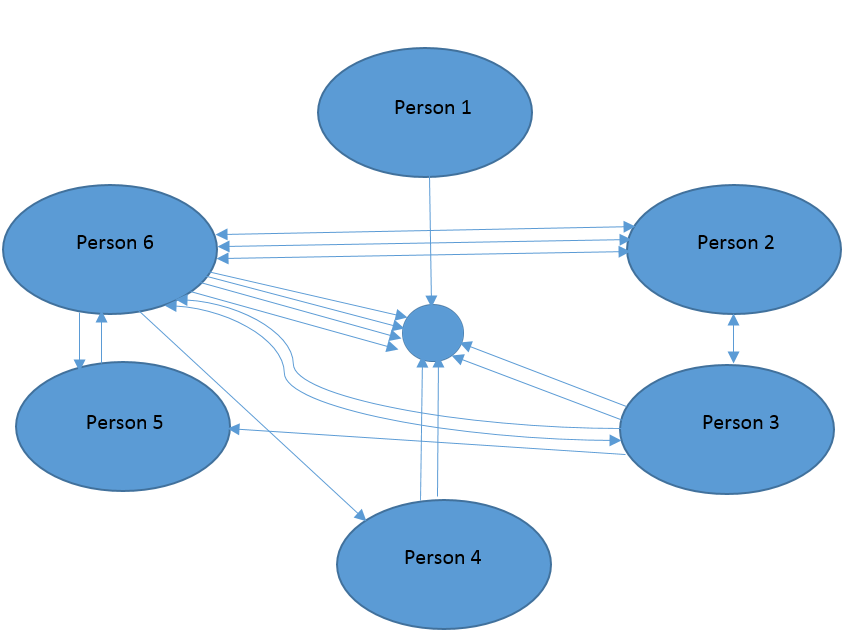
\includegraphics[scale=0.7]{gfx/sosiogram1.PNG}
    \caption{Sosiogram}
    \label{sosiogram}
\end{figure}

Person 2 og Person 6 hadde begge bakgrunn innen temaet som ble diskutert og samtalen gikk derfor mye mellom dem, mens resten hørte på. Vi kom i ettertid frem til at dette var en lite effektiv måte å jobbe på. Det ble derfor bestemt at diskusjoner som gikk på detaljnivå og hvor hele gruppens meninger ikke var nødvendig, skulle taes opp i mindre subgrupper mellom dem det gjaldt. På denne måten fikk vi bedret gruppens effektivitet og i tillegg utnyttet de ulike gruppemedlemmenes kompetanse på en bedre måte. 

\section{Gjennomføring av kreative prosesser}
De kreative prosessene i gruppen begynte i hovedsak da vi skulle velge oppgave å jobbe med. Vi brukte brainstorming til å komme frem til de fleste idéene våre. Med litt god tid til denne prosessen kom det frem mange forslag og alle fikk ytret sine meninger. Gjen\-tatte ganger ble forslag til problemstilling ikke godkjent av landsbyhøvding på grunn av simpel idé, lite realistisk eller gjennomførbar oppgave, eller problemstilling for lite relatert til robot. 

Den tredje landsbydagen måtte gruppen komme opp med en ny problemstilling siden daværende problemstilling ble litt for simpel. Flere reagerte negativt og ble litt skuffet siden de var motivert for idéen gruppen måtte bevege seg bort fra. Utfordringen her var å endre problemstillingen slik at alle gruppemedlemmene ble like fornøyd. Det hadde vært nok arbeid å komme frem til problemstillingen gruppen hadde bestemt seg for. To av gruppemedlemmene var forberedt på at gruppen kanskje måtte velge ny problemstilling, dermed hadde de litt mer positiv innstilling. Dette hjalp resten av gruppen med å komme seg videre og bli fornøyd med en ny problemstilling. 

\section{Rollebevissthet og fleksibilitet i rollevalg}
I gruppen er det et medlem som har driftet mot en lederrolle, særlig når gruppen har vært lite motivert. Denne personen påvirker gruppen med sitt fravær, eller tilstedeværelse. Gruppen har merket ved flere anledninger hvor han enten har vært borte en liten del eller hele dagen, at effektiviteten kan gå litt ned. Denne personen har hele tiden aktivt søkt tilbakemelding for å få vite hva resten av gruppen syntes om måten han ledet på og i hvilke situasjoner han tredde inn i rollen. 


\section{Effektiv beslutningstaking}
I løpet av idéfasen fant et av gruppemedlemmene ut at metoden som var planlagt å bruke for å finne posisjon eller avstand ikke var mulig for oss å implementere. Han var dermed allerede innstilt på at vi måtte endre på idéen vår når han møtte opp den dagen, noe resten av gruppen ikke var. For å få litt fortgang på arbeidet la han press på gruppen til å ta et valg, og ville ha en håndsopprekning for å avgjøre det videre arbeidet. En annen på gruppen følte at han ikke hadde fått nok tid og sa ifra. Dermed tok gruppen en pause og fikk bedre tid til å bestemme seg. Denne betenkningstiden gjorde at vi endte opp med en helt ny idé. Denne nye idéen ble grunnlaget til prosjektet sånn det endte opp. Etter at gruppen fikk oppleve hvor stor forskjell ordentlig betenkningstid kan gjøre, ble vi veldig oppmerksom på å ha nok tid før viktige avgjørelser. Om vi visste at en avgjørelse måtte bli tatt ved neste landsbydag gjorde vi det til en vane å ta opp saken på slutten av dagen, slik at vi kunne tenke på det til gangen etter.
    
Gruppen skulle på et tidspunkt avgjøre om kamerasystemet skulle brukes eller ikke. Et av gruppemedlemmene, som hadde litt mer oversikt enn andre, presenterte både for- og motargumenter for begge scenarioene. Selv om han hadde gjort seg opp en menig allerede, la han frem argumentene på en objektiv måte og forsikret gruppen om at han ville respektere flertallets avgjørelse uansett. Resten av gruppen syntes dette var en veldig ryddig og fin måte å gjøre det på og gjorde det lettere å ta en avgjørelse.

Gruppen har hele tiden vært enig om at for å bli så effektive som mulig var det viktig at alle følte eierskap til problemstillingen. Vi var derfor nøye med å, med jevne mellomrom, gjennom hele prosessen, spørre i felleskap om alle var komfortable med retningen vi beveget oss i. 
% Hoveddel

\chapter{Hoved2} % Chapter title

\label{ch:hoved2} % For referencing the chapter elsewhere, use \autoref{ch:mathtest}

%----------------------------------------------------------------------------------------

% Skrives i fortid.

% Gjengi situasjoner med forbedringspotensial. 
% Referanse til teori som kaster lys over utfordringen. 
% Reflektere over svakheter og hvordan vi kan forbedre oss, kombinert med teori. 
% Evaluere om målene ble nådd.


Alle problemer som oppsto iløpet av tiden gruppen har jobbet sammen valgte vi å løse med en metode fra en bok av  Susan Wheelan \cite[s.
61-63]{wheelan_creating_2012} som går ut på å gjenkjenne problemet, analysere problemet, ta en avgjørelse og akseptere og følge denne avgjørelsen. Dette var en metode som fungere bra for vår gruppe. I hoveddelen har vi valgt å fokusere på to hovedtema; idéavklaring og effektivitet.

\section{Idéavklaring}
Problemene til gruppen vår startet allerede i idéfasen, hvor problemstillingen skulle bestemmes. Her har gruppen vår hatt mye motgang. En problemstilling ble ikke godkjent av landsbyleder og en problemstilling samt enkelte tekniske løsninger har vi måtte forkastet pga. lite gjennomførbarhet.

Når gruppen ikke fikk godkjent første problemstillingen sin var dette fordi landsbylederen mente idéen ikke var relevant nok til landsbytemaet <<Robot og Menneske>>. De fleste på gruppen var ikke forberedt på dette i det hele tatt, og ble derfor ganske skuffet siden vi allerede hadde brukt mye tid på å forme idéen og gjort oss opp en del tanker rundt løsninger og arbeidsfordeling. To av gruppemedlemmene hadde vært litt mer forberedt på at vi kanskje måtte bytte problemstilling, og ble derfor ikke like skuffet. De hjalp resten av gruppen med å omstille seg og starte idémyldringen igjen.  

Etter at ny problemstilling var bestemt oppsto det et nytt problem. En i gruppen hadde brukt litt tid mellom to landsbydager til å finne ut mer om teknologien gruppen hadde planlagt å bruke. Han fant da ut at teknologien ikke lot seg bruke til vårt formål og han var derfor allerede klar for å bytte problemstilling når han kom til neste landsbydag. Etter litt diskusjon, for å få litt fortgang på arbeidet, la han litt press på gruppen til å ta et valg mellom et par ny problemstillinger vi hadde foreslått. Flere på gruppen følte ikke de hadde fått tid til å tenke seg godt nok om, en av dem sa ifra om dette. \todo{aksjon}Dermed tok gruppen en god pause og vi fikk mer tid til å tenke. Denne betenkningstiden gjorde at vi endte opp med en helt annen problemstilling, enn hva vi egentlig skulle ha valgt mellom tidligere. Denne nye problemstillingen ble grunnlaget for prosjektet sånn det endte opp. Etter at gruppen fikk oppleve hvor stor forskjell ordentlig betenkningstid kan gjøre, ble vi veldig oppmerksom på å ha nok tid før viktige avgjørelser. Om vi visste at en avgjørelse måtte bli tatt ved neste landsbydag gjorde vi det til en vane å ta opp saken på slutten av dagen, slik at vi kunne tenke på det til neste gang.

Gruppen måtte flere ganger ta stilling til hvilke tekniske løsninger vi skulle gå for å realisere prosjektet vårt. Vi måtte blant annet avgjøre om vi skulle bruke kamerasystemet eller ikke. For at vi skulle få tatt en avgjørelse uten at alle i gruppen brukte tid på å sette seg inn i begge alternativene, \todo{Aksjon?}lot vi ene gruppemedlemmet, som hadde litt mer oversikt enn andre, presenterte både for- og motargumenter for begge alternativene. Selv om han hadde gjort seg opp en mening allerede, la han frem argumentene på en objektiv måte og forsikret gruppen om at han ville respektere flertallets avgjørelse uansett. Resten av gruppen syntes dette var en veldig ryddig og fin måte å gjøre det på og gjorde det lettere å ta en avgjørelse.

\section{Effektivitet}

Allerede fra første dag har det vært et fokus på å holde høy effektivitet innad i gruppen, slik at jobbing utenom onsdager ble ungått. Dette ble også formalisert som et eget punkt i kontrakten som gruppen skrev i starten av perioden. I starten var det veldig mye diskusjon, noe som ofte førte til avsporinger og tulling. Dette var noe vi tidlig oppdaget gikk ut over effektiviteten i gruppen. Som en aksjon til dette problemet begynte vi å sette tidsfrister på useriøs diskusjon. Når et medlem på gruppen merket at diskusjonen begynte og bli useriøs kunne han eller hun si ifra om at dette fortsetter vi med i noen minutter til, før vi går tilbake til tema. Dette var en avgjørelse som alle var enige i og den ble dermed tatt i bruk. Litt avsporing og tulling bidrar til god gruppefølelse og gir rom for en mer avslappet atmosfære. Derfor var det ikke utelukkende negativt at dette fant sted, spesielt ikke i startfasen. 

Noen medlemmer av gruppen hadde erfaring fra arbeidslivet, og en del effektiviseringsteknikker ble derfor hentet derfra. I begynnelsen ble blant annet Scrum \cite{scrum} tatt i bruk. \todo[nolist]{Aksjon} Såkalte <<Stand-up>>-møter har også blitt benyttet av gruppen. Dette er korte morgenmøter hvor hvert medlem forteller om hva som ble gjort forrige gang, og hva som skal gjøres for dagen. Morgenmøtene har bidratt til å iverksette medlemmene på gruppen, og effektivt sørget for at hvert medlem til enhver tid har hatt noe å gjøre.

Gruppen har til tider hatt problemer med dårlig kommunikasjon. Dette har ført til at det har blitt brukt mye tid på arbeid som senere har vist seg og ikke være direkte nyttig for resultatet. For eksempel så brukte flere i gruppen mye tid på å sette seg inn i ulike stifinnings\-algoritmer som roboten skulle bruke. På et senere tidspunkt så oppdaget enkelte på gruppen at dette allerede eksisterte inne i programvare-rammeverket til roboten. Denne situasjonen kunne ha vært unngått om vi hadde en person som bedre kjente til alle funksjonene til roboten. Selve hendelsen førte til tapt tid for gruppen og nedsatt motivasjon for dem som hadde brukt tid på arbeid som det ikke var behov for likevel. 

En av hovedårsakene til nedsatt effektivitet i gruppen var at kun én datamaskin kunne kommunisere med roboten. Dette begrenset mengden med teknisk arbeid som kunne utføres samtidig. \todo{Mulig aksjon om vi hadde hatt bedre tid}Det finnes et simuleringsverktøy for roboten som kunne ha fjernet denne flaskehalsen. Hadde dette verktøyet blitt brukt, så ville helt klart effektiviteten ha økt på sikt, men man ville brukt mye tid på å sette seg inn i dette. Med tanke på at prosjektetperioden var så kort ville det trolig ikke vært lønnsomt i vårt tilfelle. Gruppen kom derfor frem til at simuleringsverktøyet skulle nedprioriteres.

I løpet av arbeidsperioden som gruppen har vært gjennom, har det vært tydelig at engasjement og motivasjon er en viktig faktor for effektivitet. En kunne observere en klar nedgang i effektiviteten da gruppen ble nødt til å endre kurs som en følge av råd fra veileder. 




% Resultater

\chapter{Resultater} % Chapter title

\label{ch:resultater} % For referencing the chapter elsewhere, use \autoref{ch:resultater}

%----------------------------------------------------------------------------------------

% Skrives i fortid.

I dette kapittelet blir resultater som har kommet frem i løpet av prosjektperioden presentert. Gruppen har blant annet tatt personlighets\-test og en felles øvelse om samarbeid, i tillegg til å skrive personlig logg underveis i prosjektperioden. Her kommer det frem hvordan gruppen har utviklet og tilpasset seg i forhold til resten av gruppen.

% Personlige refleksjoner / Forholdet til EiT / Hva dere har lært som enkeltpersoner. 

% Sees f.eks. opp mot hva som ble presentert om hver enkelt i innledningen. Dette er tema hvor vi sensorer ikke kan sammenligne dere med forventninger, sammenligne dere med hverandre, eller sette karakter på dere. Det er flott hvis det kommer frem noe interessant, men ikke gjør slike kapitler til pliktløp, og (vær så snill!) ikke lag kapitler fylt med svada.

\section{Personlighetstyper og roller i gruppen}

Omtrent halvveis gjennom prosjekttiden hadde vi en rolleøvelse i gruppen. Hensikten med denne øvelsen var å bevisstgjøre hverandre på hvilken rolle hver enkelt av oss hadde. Grafisk fremstilling av øvelsen kan sees i \autoref{ch:roller}, der hver figur tar for seg poengene som én person fikk, inkludert personens poeng til seg selv.

På eget initiativ gjennomførte gruppen den velkjente <<Myers-Briggs Type Indicator>>-testen for å kartlegge hvilke personlighetstyper gruppen besto av. Vi endte opp en ENFJ, en ENFP, en ISFJ og tre ISTJ.

I rolleøvelsen kom det klart frem at alle i gruppen så på gruppemedlemmet med ENFP personlighet som den personen som tok mest ledelse og generelt satt mye preg på gruppen. Samme gruppemedlem kom også klart ut som den i gruppen som var minst underkastende og som utfordret andres ideer mest. En person med ENFP personlighet er sosial, nytenkende og opptatt av harmoni og godt samarbeid i gruppen, og passer derfor ofte godt som leder. Dette gruppemedlemmet var også gruppens eneste oppfattende person og er derfor mer opptatt av prosessen enn målet. Selv om resultater selvsagt er viktig for en leder, så kan for stort fokus på resultatet føre til hastet arbeid av dårlig kvalitet. Derfor bør ofte en god leder være opptatt av prosessen, noe som styrker vår tro om at riktig person opptrådte som leder i gruppen vår.

Vi hadde et tydelig skille i personlighetstyper i gruppen vår. På ene siden hadde vi en av type ENFJ og en av type ENFP som er utadvente, nytenkende og opptatt av godt samarbeid. På andre siden hadde vi tre av type ISTJ og en av type ISFJ som gjerne er litt mer stille, faktaorienterte og målrettet. I øvelsen kom det frem at de to med ekstroverte personlighet var de som tok mest av gruppens oppmerksomhet, både på godt og vondt. De introverte var jevnt over dem som i øvelsen som scoret høyest på å innordne og underkaste seg, være taus eller stille. Dette resultatet kom ikke som noe overraskelse på gruppen, siden det ligger langt mer i en ekstroverts natur å være gruppens midtpunkt, enn hva det gjør for en introvert.

Når det kom til hvem i gruppen som var sosial og bidro til å skape hygge og trivesel, fikk alle i gruppen god score. Likevel pekte gruppemedlemmet med ENFJ personlighet seg ut som den mest sosiale, og som bidro mest til trivselen i gruppen. Dette er en rolle som ofte faller naturlig for en med ENFJ personlighet. 

Øvelsen viste oss også at alle i gruppen hadde gitt ganske lik poengsum til seg selv som det de andre i gruppen hadde gitt en. Det viser at våre oppfatninger av oss selv i gruppen samsvarer med andres oppfatninger. Vi tror at ved å ikke ha noen vrangforestillinger av våre egne roller i gruppen, så har vi unngå en del konflikter som ellers kanskje ville oppstått.

\section{Samarbeidsindikatoren}
I løpet av prosjektperioden ble det tatt en undersøkelse tre ganger; en ved start, midten og ved slutten av prosjektet. Resultatet viste i hvilken grad disse faktorene ble nådd, se \autoref{samarbeidsindikatoren}. Ser på figuren at resultatene stort sett sank utover i perioden. Det er viktig å merke seg at to forskjellige gruppemedlemmer var borte henholdsvis andre og tredje gangen. Vi tror dette har påvirket resultatet, særlig tredje gangen. 
\begin{figure}[!h]
    \centering
    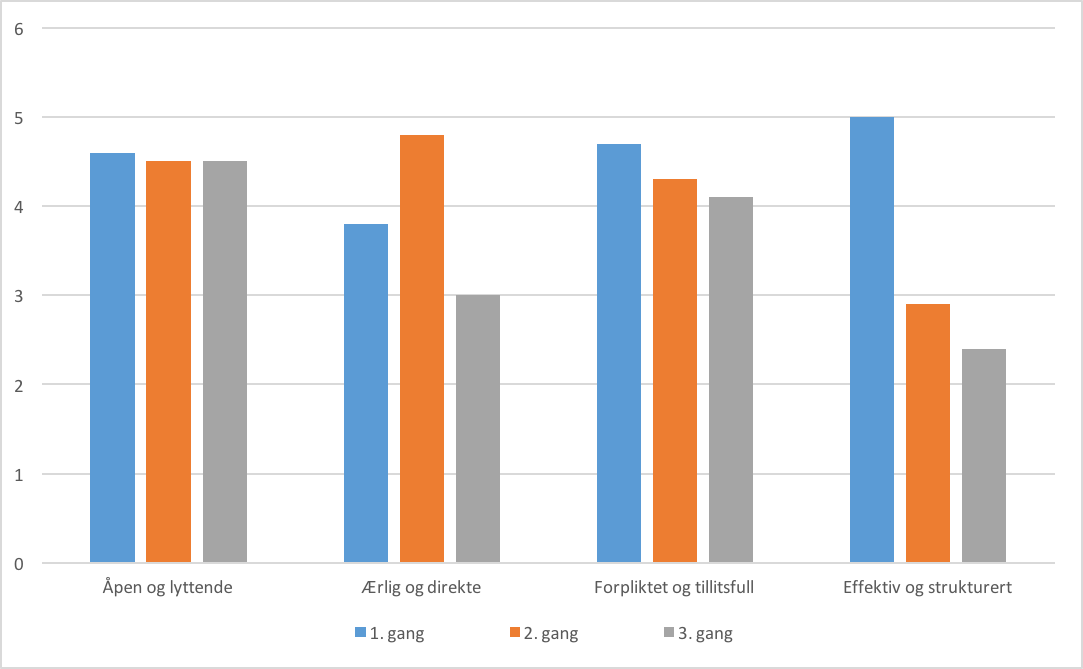
\includegraphics[width=1\textwidth]{gfx/samarbeidsindikatoren.png}
    \caption{Samarbeidsindikatoren}
    \label{samarbeidsindikatoren}
\end{figure}

Hvis vi fokuserer på <<Ærlig og direkte>>, så har den sunket den gangen den mest direkte personen på gruppen var borte. Dette må være grunnen til at den har sunket til der den endte. Vi mener selv at vi alltid har vært like ærlige og direkte mot hverandre, selv om figuren kanskje ikke viser det. I løpet av perioden har effektiviteten kanskje gått litt ned i perioder. I starten kom gruppen godt i gang og var produktive. Da den andre undersøkelsen skulle tas var vi litt skuffet og ikke fornøyd med hvor langt vi hadde kommet i forhold til målet med prosjektet, derav lavt resultat på <<Effektiv og strukturert>>. Gruppen hadde fått litt mer motgang enn forventet. For noen gruppemedlemmer forsvant ikke denne motgangen og påvirket også den tredje undersøkelsen. Personen som var borte tredje gangen var han som jobbet mest med det tekniske og hadde vært mye mer effektiv og produktiv enn hva de andre på gruppen fikk inntrykk av. Siden de fleste på gruppen hadde lite å gjøre med det tekniske utover i prosjektperioden, følte de at de ble mindre effektive, selv om de fikk jobbet mye med rapportene eller andre ting som kunne være til hjelp for prosjektet. Vi mener dette senktet den oppfattede effektiviteten og kunne realistisk sett ligget et sted mellom første og andre gang. 

Hvis man sammenligner gruppens arbeid mot Roger Schwarz sin bok om fasilitering, i kapittelet <<What Makes Groups Effective>> \cite[s. 17-34]{schwarz_skilled_2002}, er det flere sammenhenger som tyder på at effektiviteten i gruppen ble slik som resultatet viser. I starten var gruppen mer definert med hver sine oppgaver, det var et tydelig mål, alle var motivert og følte eierskap til problemstillingen. Etter å ha byttet idé et par ganger ble det målet som i starten var felles, mer en person sitt mål som resten av gruppen fulgte. Dette var mindre motiverende for resten av gruppen når de ikke lenger var like mye med på målet gruppen hadde satt seg. Dette førte til mindre gruppestruktur og resulterte i lavere effektivitet. 

\section{Personlige refleksjoner}
\subsection{Jon}

% Gruppedynamikk har fascinert meg lenge, spesielt etter jeg skrev bacheloroppgave i 2013. Vi var tre gutter som jobbet sammen, hvorav de to andre på gruppen kjente hverandre fra før. Vi leverte et godt resultat, men veien dit var fylt med personlige konflikter, dårlige tilbakemeldinger og uheldige forsvarsmekanismer. Dette er ting jeg på den tiden tenkte mye over, som jeg merket ødela for motivasjonen til arbeidet, og som kunne gjort prosjektet enklere hvis jeg og de andre på gruppen hadde oppført oss annerledes. Videre ble jeg ble spurt om hva slags grupperolle jeg tar under et jobbintervju senere i 2013. Jeg føler jeg svarte godt for meg på tidspunktet, men skjønte senere at jeg ville lære mer om dette da jeg hørte hva EiT gikk ut på. Ellers kan kunnskapen brukes i det personlige livet, enten i familie, bofellesskap eller med kjærester. 

% Etter fem år med høyere utdanning preget av mye gruppearbeid har jeg begynt å se trender på hva slags rolle jeg tar i grupper. Under EiT har jeg hatt forventninger til å sette ord på flere av disse trendene, bli mer kritisk til hva jeg kommuniserer både med det jeg sier og det jeg ikke sier, og å lære om hvilke handlinger som er rette å gjøre i dilemmaer hvor to sider av en konflikt har gode poeng om hvorfor de har rett. 

Jeg ser på meg selv som en utadvent person, og dette har også blitt bekreftet fra inntrykk jeg har mottatt i gruppen. Det var viktig for meg å bli kjent med alle i gruppen fra starten, spesielt siden jeg gikk glipp av første landsbydag. Det er den sosiale rollen jeg etterhvert festet i gruppen jeg føler er mest interessant å reflektere over. Den sosiale rollen er et produkt av at jeg engasjerer meg med innspill i diskusjoner om arbeid, gir tilbakemeldinger, er en god lytter, opptatt gruppemedlemmers velvære og er en bidragsyter under pauser og i lunsjen. Jeg prøver å ha fokus på å få med alle, det betyr for eksempel at jeg eksplisitt spør de minst deltagende om deres mening. Til tross for dette er det noen jeg har fått bedre kontakt med på gruppen, som jeg automatisk gir litt mer oppmerksomhet. Jeg synes det er viktig å balansere ris og ros, og har fokus til på å bidra mot dette. Dette er noe som funker mye i mitt daglige liv, som jeg har fortsatt med i prosjektarbeidet og gjennomført i varierende mengde. Ros øker mestringsfølelsen til mennesker, og kan virke motiverende. I praksis er det ofte enklere å kritisere noen for noe de har gjort feil eller ikke gjort, heller enn noe som oppfyller forventninger eller er gjort bra.

En betydelig bieffekt av rollen min i gruppen er at jeg tar opp mye oppmerksomhet. Dette er selvsagt på godt og vondt, men sett over hele prosjekttiden har det nok vært mest negativt. I startfasen mens vi diskuterte problemstilling kunne jeg fort gi et ironisk svar på idéer som uansett kanskje virket litt for oppfinnsomme. Denne ironien kunne så bli misforstått som videre førte til bortkastet tid. Jeg er nok også en av de i gruppen som bidrar til flest avsporinger. Selv om flere enn meg skal ha skyld for unødvendige avsporinger, sitter jeg med en følelse av at jeg har brakt frem en evne til hyppigere avsporinger hos mennesker som vanligvis kanskje ikke sporer av så ofte. Dette er en interessant karakteristikk, og noe jeg tar med meg videre. Som følge av dette burde jeg se an situasjonen og generelt forholde meg helt seriøs, og spare vitser, historier og andre temaer som ikke passer under arbeid til lunsj og pauser. Dette er det viktig at jeg får endret på.

En annen konkret atferd som har hatt noe å si for gruppa er mengden tid jeg bruker på å være for sen. Jeg kommer ofte fem minutter for sent til arbeidsdagen, og dette forsinker ikke bare gruppa til rommet hvor vi skal jobbe, men det kan også skape irritasjon eller forstyrre arbeidspsyken som noen bygger seg opp. Bakenliggende årsaker for at jeg kommer for sent til arbeidet når jeg klarer å rekke busser, jobb og andre litt mer definerte avtaler og obligatoriske tidspunkt kan være fordi jeg ikke prioriterer arbeidet nok i hodet mitt. I tillegg finnes det rom i reglene som ikke straffer mindre forsinkelser. Forsinkelsene mine har blitt tatt opp flere ganger i gruppa, og jeg ønsker å bli flinkere på dette, og burde lære meg å gi tilsvarende settinger høyere prioritet.   

Når det kommer til arbeid med prosjektet er jeg fornøyd med egen innsats, mindre fornøyd med egen konkret leveranse. Jeg tok tidlig på meg ansvaret for dokumentasjon og papirer, som en slags sekretær i gruppa. Dette var også i henhold til samarbeidsavtalen. Jeg skrev mesteparten av grupperefleksjonene, men var til stadighet ikke helt fornøyd hvordan de ble sammenlignet med eksempelrefleksjonen. Videre prøvde jeg hele tiden å engasjere meg i arbeidsoppgaver hvis jeg ikke hadde noe å gjøre. Eksempelvis prøvde jeg å paralellisere arbeidet i større grad ved å få opplæring og bidra med mine kunnskaper i programmering, men det viste seg at det ble vanskelig på grunn av feilmeldinger og bugs som oppstod. Da falt jeg tilbake på å skrive rapport eller lese teori. 

Jeg er fornøyd med måten jeg møter kritikk på, spesielt i en setting som EiT. Hvis mennesker gir tilbakemeldinger på en konstruktiv måte er jeg veldig tilbøyelig for å høre på og ta det til meg. Mitt mål er å bli verdsatt av gruppemedlemmene mine, slik at de kan ha tillit til å delegere arbeid til meg, eller ta på seg arbeid for meg.

\subsection{Harald}
Da jeg først fikk vite om emnet Eksperter i Team ble jeg interessert i hvilken landsby jeg ville ende opp og hvem jeg kom til å jobbe sammen med en gang i uken i løpet av et semester. Jeg fikk den samme følelsen som jeg har fått når jeg skal begynne i en ny klasse på en ny skolen, det var litt spennende. I starten av prosjektperioden var jeg motivert til å lære mye om meg selv i en gruppesammenheng i tillegg til å utforske muligheter rundt temaet om roboter i samfunnet. Førsteinntrykket til Eksperter i Team var bedre enn forventet. Siden jeg er en anelse sjenert, særlig rundt nye mennesker, var jeg litt stille i starten. Dette var også fordi noen andre på gruppen hadde en tendens til å prate mye, og førte til at jeg ikke helt kom på samme plan som andre i gruppen. Etter noen ganger fikk gruppen balansert seg litt og samtalen ble bedre fordelt utover flere parter. 

En ting som jeg angrer litt på er at jeg ikke satte meg mer inn i det tekniske på starten. Siden det var ukjent og andre på gruppen hadde kommet mer igang, trakk jeg meg litt tilbake og lot andre jobbe med det. Dette førte til at jeg gikk glipp av muligheten til å arbeide med det tekniske. Noe jeg har merket mer prosjektarbeid i gruppe er at jeg kanskje bryr meg mer om å møte opp og være tilstede enn å være produktiv. Jeg følte til tider at jeg ikke fikk gjort så mye som jeg burde. Dette har også litt med det at vi hadde udefinerte arbeidsoppgaver. Utover i perioden lot jeg meg kanskje irritere litt over småting, som at noen ofte var sene om morgenen. Det var lett å glemme slike små ting når man ser på helheten. Jeg var generelt veldig fornøyd med samholdet i gruppen, og føler jeg har lært mer om hvordan jeg fungerer i et team.

\subsection{Erlend}
Jeg hadde egentlig ikke så mange forventninger når jeg begynte med Eksperter i Team. Landsbyen jeg havnet i, Robotikk og Menneske, var andrevalget mitt. Førstevalget var byggelandsbyen, dette fordi jeg generelt liker å jobbe med praktiske ting. Jeg hadde hørt fra andre om at kvaliteten på emnet i hovedsak var avhengig av hvilken gruppe en havnet på. Derfor var det gledelig at jeg allerede fra første dag hadde et positivt inntrykk av de jeg kom på gruppe med. Jeg likte det faktum at vi var en ren teknisk gruppe med forholdsvis like studie\-retninger. Jeg så på dette som en fantastisk mulighet til å kunne lage noe spennende sammen. Personene på gruppen virket også engasjerte og motiverte i forholdet til emnet. Samtalen fløt også lett, og det var ikke noe problem med å få sagt sin mening til en hver tid. 

Selv så har jeg aldri betraktet meg selv som en lederperson. Samtidig så har jeg heller aldri har vært avhengig av at folk må fortelle meg hva jeg skal gjøre til en hver tid. Jeg liker å delta aktivt i de avgjørelsene som blir tatt, og ikke bare passivt si meg enig i det andre mener er den beste avgjørelsen. Jeg har derfor på flere tidspunkt i løpet av dette emnet vært i opposisjon på en del store avgjørelser. Nå i ettertid ser jeg at dette er en rolle som jeg kunne ha inntatt i enda større grad. Jeg kom nemlig med en god del kritikk til å bruke Motion-Capture systemet i forbindelse den autonome handlevognen. Jeg påpekte at tiden for gjennomføre et slikt prosjekt var for liten, og at oppgaven dårlig lot seg dele opp. Nå i ettertid har det vist seg at mitt sistnevnte argument har vært et stort problem for gruppen. Oppgaven vi landet på var vanskelig å dele opp, noe som førte til at effektiviteten gikk betydelig nedover. 

Rent jobbmessig så er jeg helt greit fornøyd med min egen innsats. Jeg er kun misfornøyd med at jeg ikke har fått bidratt så mye med det jeg er virkelig god på. Eksperter i Team har først og fremst lært meg hvor viktig det er å ytre sin mening, spesielt hvis det er noe man sitter å brenner inne med. Dine argument er vel så gode som alle andres, og det er derfor så utrolig viktig å få diskutert dem. 

\subsection{Håvard}
Jeg gikk inn i Eksperter i Team med positive forventning og var veldig spent på hvordan jeg kom til å fungere med en helt ny gruppe mennesker. Opp i gjennom studietiden har jeg vært bundet til grupper jeg allerede kjente fra før, så å kunne møte nye folk i en helt ny gruppe ville bli spennende. Jeg har en veldig skeptisk og realistisk holdning, dette var noe jeg håpet ikke ville være i veien for andre hvis de prøvde å strekke seg etter noe jeg mente var urealistisk. Men dette var ikke noe problem i vår gruppe da alle delte denne samme holdningen. Jeg er vant med å måtte lede litt, eller ihvertfall å få folk litt i gang med oppgaver, men denne gangen var jeg den som trengte å bli litt satt i gang. Dette var en helt ny erfaring for meg, og var veldig interessant. Jeg har følt at jeg har blitt bedre kjent med meg selv. Jeg fikk også oppleve at mitt humør kan gå ut over andre, og dette er noe jeg har prøvd å jobbe med mer i ettertid. Rent jobbmessig er jeg ikke spesielt fornøyd med egen innsats, jeg føler jeg kunne ha vært litt mer frempå slik at det kunne blitt mindre jobb for andre. Dette er noe vi har reflektert mye over mot slutten og blitt enig om at kunne vært annerledes. Alt i alt er jeg fornøyd og synes dette har vært en lærerik erfaring og ta med seg videre i livet og inn i arbeidslivet.

\subsection{Helene}
Jeg hadde allerede fra starten en positiv holdning til emnet. Jeg var spent på hvem jeg kom til å komme på gruppe med, men tenkte at emnet kom til å bli anderledes og interessant uansett. Gjennom mine fire år her på NTNU har jeg hatt mye gruppearbeid, likevel har jeg, som mange andre, ofte jobbet med de samme personene hver gang. Dette har gjort at jeg jobber veldig bra sammen med disse, men har fått lite trening å å forholde meg til nye mennesker. Jeg har heller ikke særlig erfaring med å jobbe i grupper på størrelsen med den vi har hatt i dette emnet. Jeg syns Eksperter i Team gir en mer realistisk opplevelse av hvordan et gruppearbeid foregår i arbeidslivet, noe jeg setter stor pris på å få øvd meg litt på. Jeg sitter igjen med følelsen av å ha lært mer om min innvirkning på en gruppe og at jeg vet mer om hva jeg kan gjøre for å bidra til å få et så effektivt gruppearbeid som mulig. Det har vært fint å hatt et emne hvor man har tid til å reflektere over gruppearbeidet og ikke bare haste i mål. Jeg tror jeg kommer til å få bruk for erfaringene jeg har fått gjennom Eksperter i Team når jeg kommer ut i arbeidslivet. 

Faglig føler jeg meg helt klart sterkest på teori og følte derfor ikke jeg hadde så veldig mye å bidra med på det praktiske som ble gjort. Likevel følte jeg at jeg var flink til å finne andre oppgaver som jeg var mer komfortabel med å gjøre. Jeg er derfor fornøyd med egen arbeidsinnsats.

\subsection{Morten}
Landsbyen, Robotikk og Menneske, var for min del andrevalget jeg søkte på. Jeg gikk likevel inn i emnet med åpent sinn, og forventning om at vi kunne få til noe interessant og givende. Tidlig i arbeidet følte jeg at vi hadde fått satt sammen en god gruppe, med komplementerende personligheter og erfaringsgrunnlag.

I gruppen tok jeg ganske tidlig en noe ledende rolle. Vi ble enige om å benytte tankegang fra såkalt smidig utvikling, eller Scrum\footnote{\url{http://en.wikipedia.org/wiki/Scrum_(software_development)}}, der man benytter seg av korte utviklingsintervall og tydelig definerte delmål. I dette paradigmet har man en <<Scrum Master>>, som har som rolle å fjerne utvendige hindringer som står i veien for gruppens fremgang, og generelt fungere som en buffer mellom gruppen og ytre forstyrrelser, i tillegg til å sørge for at gruppen har tilstrekkelig fremgang til å møte de kravene som stilles av ledelsen. Personen har ingen formell autoritet, men har en rolle som er beskrevet som en blanding av å være både gruppens leder og tjener, samtidig som man også arbeider med oppgaver på linje med de andre i gruppen. Dette har vært en ny rolle for meg, noe som har vært spennende. Det har derfor vært en god trygghet å kontinuerlig få tilbakemelding fra resten av gruppen om hvordan de har opplevd min rolle.

Som en følge av denne rollen har jeg i blant brukt ekstra tid for å sette meg inn i problemer som har vært til hinder for gruppens fremgang. En konsekvens av dette er at jeg har sittet på kompetanse ingen andre i gruppen har hatt. Vi har brukt noe tid på å spre denne kunnskapen, men kanskje ikke nok. Som en konsekvens føler jeg at gruppens effektivitet innen enkelte oppgaver har vært litt for avhengig av om jeg har vært tilstede eller ikke. Dette er nok en utfordring man møter i mange arbeidssituasjoner, og jeg skulle nok likt å vite mer om hvordan man håndterer det på en god måte.

Rollen jeg beskriver ovenfor, i sammenheng med at jeg er en forholdsvis utadvendt person, har ført til at jeg har vært fremtredende i diskusjonene i gruppa. Dette er noe det er viktig for meg å være bevisst på, slik at også de som ikke er like på hugget til å ta ordet får komme til. Emnet har gitt meg nyttig trening i nettopp dette. Ingen i gruppa har gitt meg tilbakemelding på at de har følt seg overkjørt, heller ikke på direkte spørsmål, og det tar jeg som en indikasjon på at jeg har funnet en god balanse.
% Diskusjon

\chapter{Diskusjon} % Chapter title

\label{ch:diskusjon} % For referencing the chapter elsewhere, use \autoref{ch:mathtest}

%----------------------------------------------------------------------------------------

% Skrives i fortid.

% Bare hvis dere har noe mer å diskutere, men det tar seg alltid godt ut å være kritisk til eget arbeide her.

% Burde kanskje ha dratt inn pensum i arbeidet.

% Hvorfor er dette faget bra?
% - Eksempel med rollebevissthet i jobbintervju f.eks.


Gruppen brukte mye tid i starten på å finne en problemstilling som engasjerte alle gruppens medlemmer og hvor alle følte de fikk brukt sin kompetanse. Både første og andre idé ble avslått av ulike årsaker. Dette førte til at gruppen begynte å føle et tidspress for å komme igang med arbeidet og at problemstillingen vi endte opp med ble fattet på et litt dårligere grunnlag enn hva de foregående problemstillingene hadde blitt. Alle i gruppen var engasjerte for idéen, men kompetansen til gruppen ble ikke like godt ivaretatt. 

Når arbeidet startet tok et av gruppemedlemmene fort styringen på det tekniske. Dette gruppemedlemmet fikk naturlig nok mest kunnskaper om systemet vårt og for å spare mest mulig tid ble det han som jobbet videre med det tekniske hver gang, mens resten tok for seg andre oppgaver. Dette var en avgjørelse gruppen i ettertid har diskutert og kommet frem til at var en dårlig løsning. Selv om det, der og da, var mest effektivt og la den med mest kunnskaper gjøre jobben, så gjorde vi oss selv veldig sårbare som gruppe ved å være så avhengig av én person. Det kom frem at dette var noe de fleste i gruppen hadde tenkt på uten å si noe, men innen vi tok det opp i gruppen, var det gått såpass lang tid at å lære opp andre gruppemedlemmer i programvaren ville ta for lang tid. Vi hadde alle sammen hatt en litt for passiv holdning til problemet. Dette kan ha noe med at ikke alle på gruppen følte de hadde like mye å bidra med på det tekniske etter at vi måtte bytte problemstilling. 

Som gruppe burde vi nok kanskje stoppet litt mer opp før den endelige problemstillingen ble bestemt. Vi kunne da kanskje innsett tidsnok at kompetansen som skulle til for å løse oppgaven var mer skjevt fordelt blant gruppemedlemmene med denne problemstillingen enn med de tidligere forslagene. Vi kunne også vært flinkere til å si rett ut at vi syntes arbeidsfordelingen ikke var helt som ønsket, slik at vi kunne vært flere på den tekniske delen fra starten. 

Gruppen ble tidlig i idemyldringsfasen opphengt i at resultatet skulle bli noe som fungerte i praksis. Denne tanken var noe som motiverte alle og vi så derfor på dette som viktig å få gjennomført. Vi kunne kanskje valgt å ikke fokusere så sterkt på dette, noe som kunne ført til at vi hadde kommet opp med flere ideer som lot seg gjennomføre på en mer effektiv måte enn den vi endte opp med. 

Det at gruppen har vært ganske faglig homogen kan ha vært med å påvirke gruppearbeidet vårt. I David Johnson og Frank Johnson sin bok om grupper, i kapittelet <<Valuing diversity>> \cite[s. 452-453]{johnson_joining}, blir det nevnt flere ulemper med homogene grupper. Uenigheter og motstridende perspektiv i en gruppe er ofte en god måte å komme frem til best mulig avgjørelser og for å fremme kreativ tenkning. I en homogen gruppe risikerer man at gruppemedlemmene tenker for likt og dermed går glipp av spennende innspill man ellers ville fått. Homogene grupper unngår oftere å ta sjanser og går dermed glipp av muligheter til å øke produktiviteten. De inngår oftere i gruppetenkning \cite{groupthink}, noe som kan føre til dårlige avgjørelser. Siste som ble nevnt i teksten var at homogene grupper fungerer best i statiske situasjoner og har større vanskeligheter for å tilpasse seg endringer. Det er naturlig nok vanskelig å vite hvordan vi ville vært som gruppe om vi hadde hatt et større faglig mangfold, men vi syns det er grunnlag for å tro at en del kunne vært anderledes. Vi hadde nok vært mindre ensporet under idemyldringen og generelt fått flere friske og nytenkende innspill i diskusjonene våre, noe som fort kunne ført til andre avgjørelser enn hva vi endte opp med. Vi hadde til tider litt problemer med å omstille oss når vi f.eks. måtte bytte problemstilling. Hadde vi hatt et større mangfold på gruppen kunne det kanskje ha hjulpet oss til å raskere komme oss videre. Vi føler ikke at mangel på faglig mangfold har ført til dårlige avgjørelser, men vi tror større mangfold kunne fått oss til å bli mer nytenkende og til å ta flere sjanser. 


% Konklusjon

\chapter{Konklusjon} % Chapter title

\label{ch:konklusjon} % For referencing the chapter elsewhere, use \autoref{ch:mathtest}

%----------------------------------------------------------------------------------------

% Dere bør ha en konklusjon, bare for å runde av rapporten. Referer forbedringene deres kort som minimum, men gjør det kort hvis dere ikke har mer å konkludere med.

% Har ambisjonene og forventingene til faget blitt møtt? Lært noe? Hva eller ikke, og hvorfor / ikke. 

Jevnt over semesteret har vi hatt god stemning og et godt sam\-arbeid i gruppen. Vi har ikke hatt noen hendelser som har krevd store endringer i gruppen, men vi har gjort noen små justeringer der vi har sett et forbedringspotensiale. Vi ha blitt mer tydelig på morgenmøter om hva man har gjort og hva man skal gjøre, for å unngå at noe blir gjort to ganger. Vi har blitt flinkere til å ta ordentlig betenkningstid før viktige avgjørelser, slik at man ikke bare føler strømmen. Vi har blitt flinkere til å kun involvere dem i gruppen som trenger å bli involvert i en diskusjon, noe som frigir resten av gruppen til å jobbe videre med sitt arbeid. Vi har også blitt bedre på å sette en begrensing på avsporinger og tull.

Vi har alle i gruppen jobbet en del med gruppearbeid tidligere, men vi syntes likevel at emnet har vært nyttig. Eksperter i Team har gitt en mulighet til å fokusere på selve gruppearbeidet på en helt annen måte enn normalt gruppearbeid gjør. Normalt vil man ha så stort fokus på oppgaven som skal gjøres at man glemmer litt å tenke på hvordan man jobber sammen. Vi har igjennom emnet lært mer om hva som gjør en gruppe effektiv og hvordan vi kan gjøre justeringer på måten vi arbeider på for å bli mer effektive. Vi har fått erfare hvordan det er å jobbe samme i et team med andre som ikke har helt lik bakgrunn som en selv. Vi har også fått oppleve viktigheten med god kommunikasjon i en gruppe. Emnet har gjort oss mer reflekterte, noe vi tror vil gjøre oss til bedre gruppemedlemmer i fremtiden. 


%----------------------------------------------------------------------------------------
%	THESIS CONTENT - APPENDICES
%----------------------------------------------------------------------------------------

\appendix

\part{Vedlegg} % New part of the thesis for the appendix

\chapter{Roller}
\label{ch:roller}

\begin{figure}[!ht]
\centering
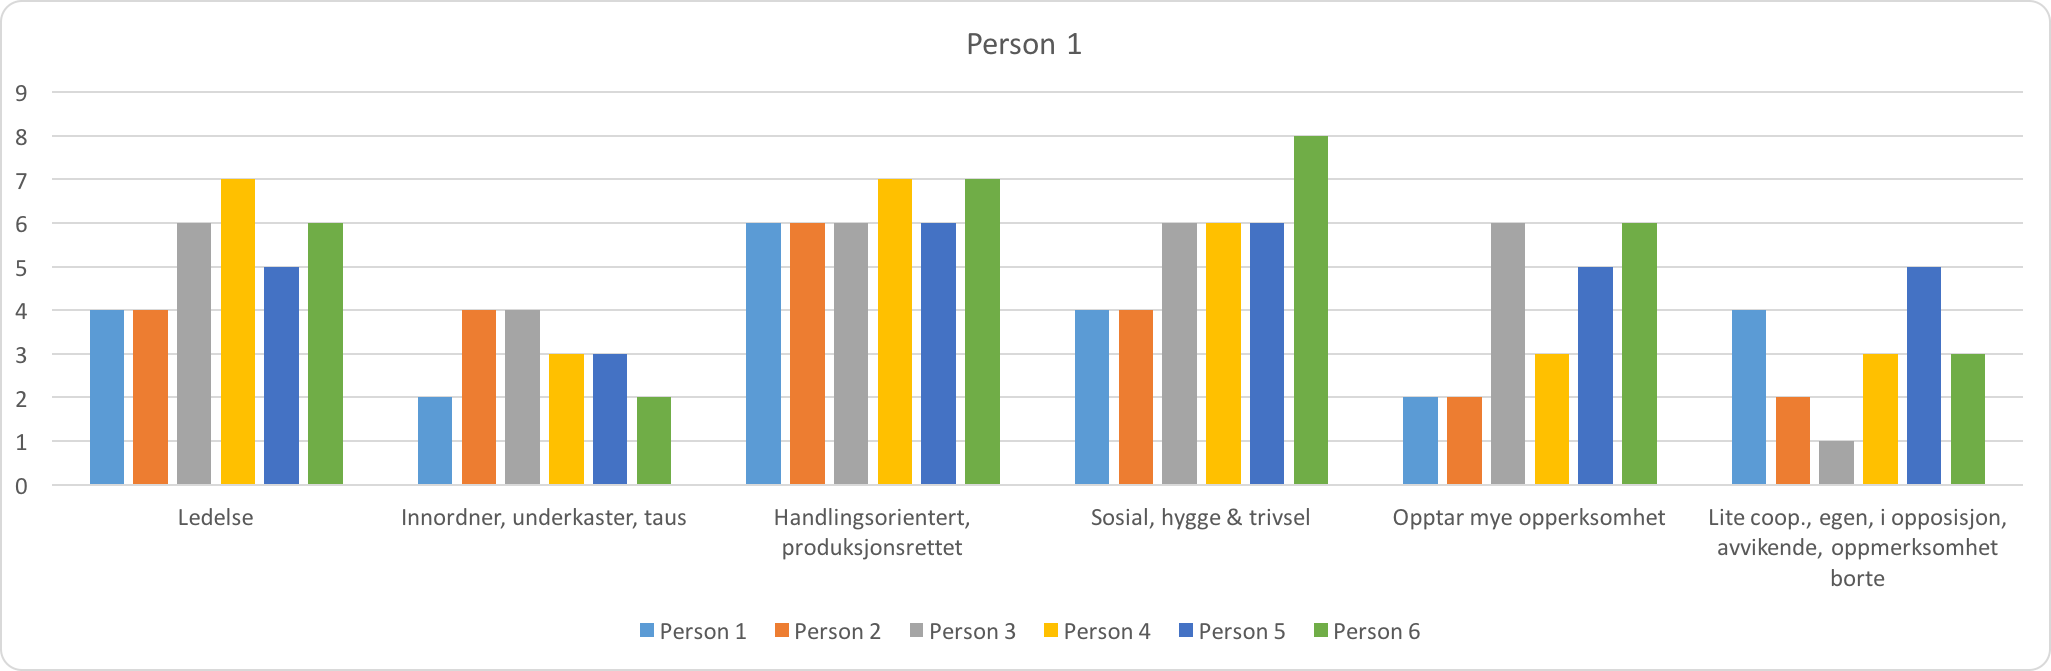
\includegraphics[width=1\textwidth]{gfx/roller_person1.png}
\caption{Roller – Person 1}
\label{roller_person1}
\end{figure}

\begin{figure}[!ht]
\centering
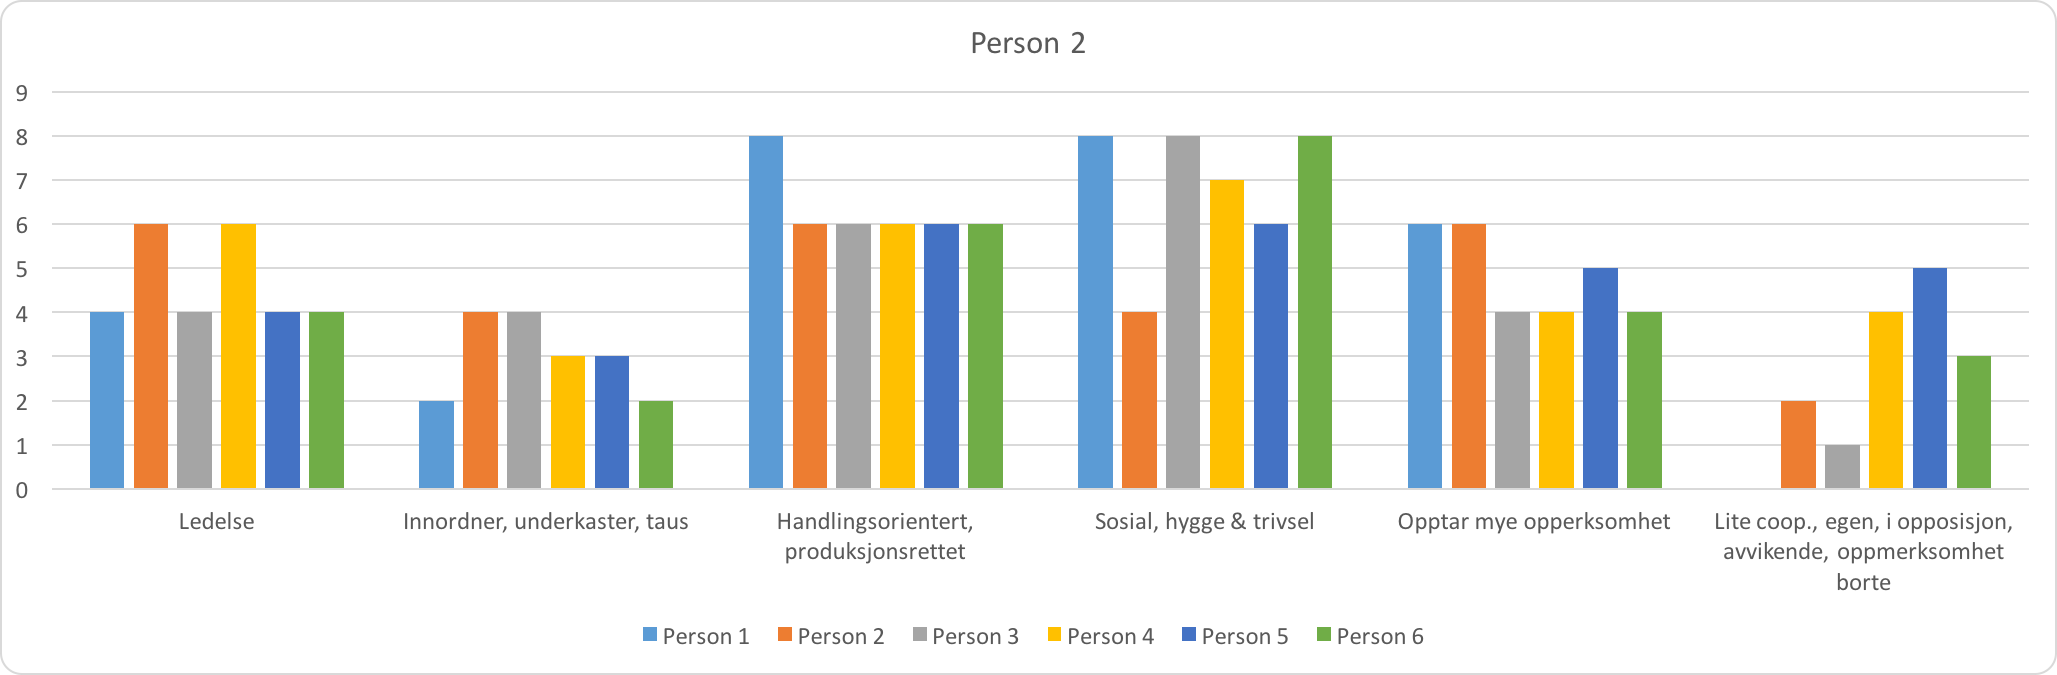
\includegraphics[width=1\textwidth]{gfx/roller_person2.png}
\caption{Roller – Person 2}
\label{roller_person2}
\end{figure}

\begin{figure}[!ht]
\centering
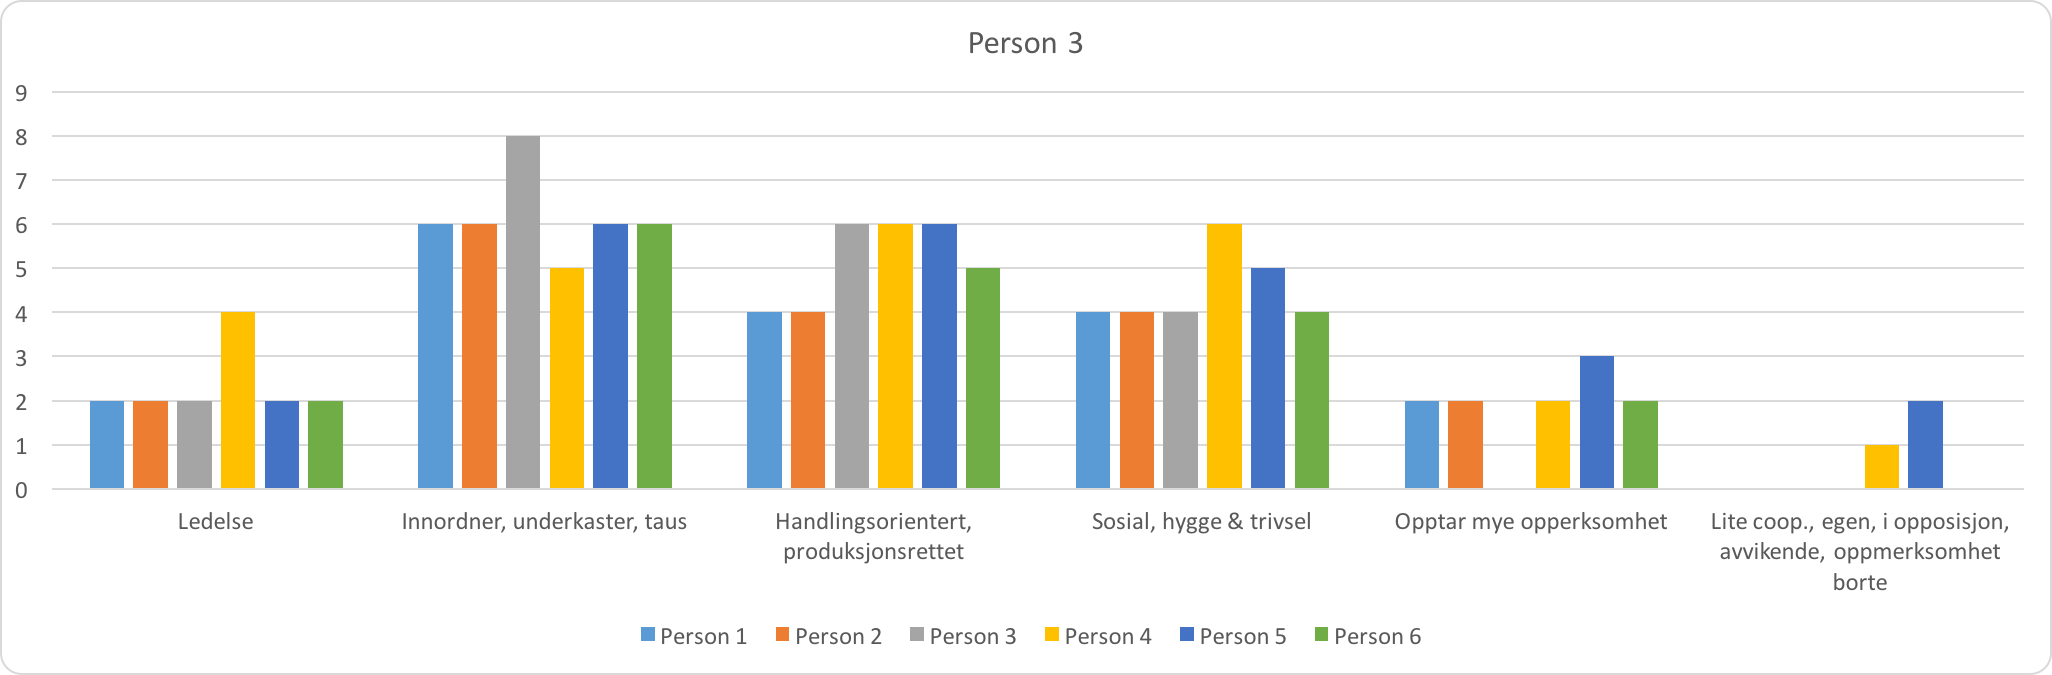
\includegraphics[width=1\textwidth]{gfx/roller_person3.png}
\caption{Roller – Person 3}
\label{roller_person3}
\end{figure}

\begin{figure}[!ht]
\centering
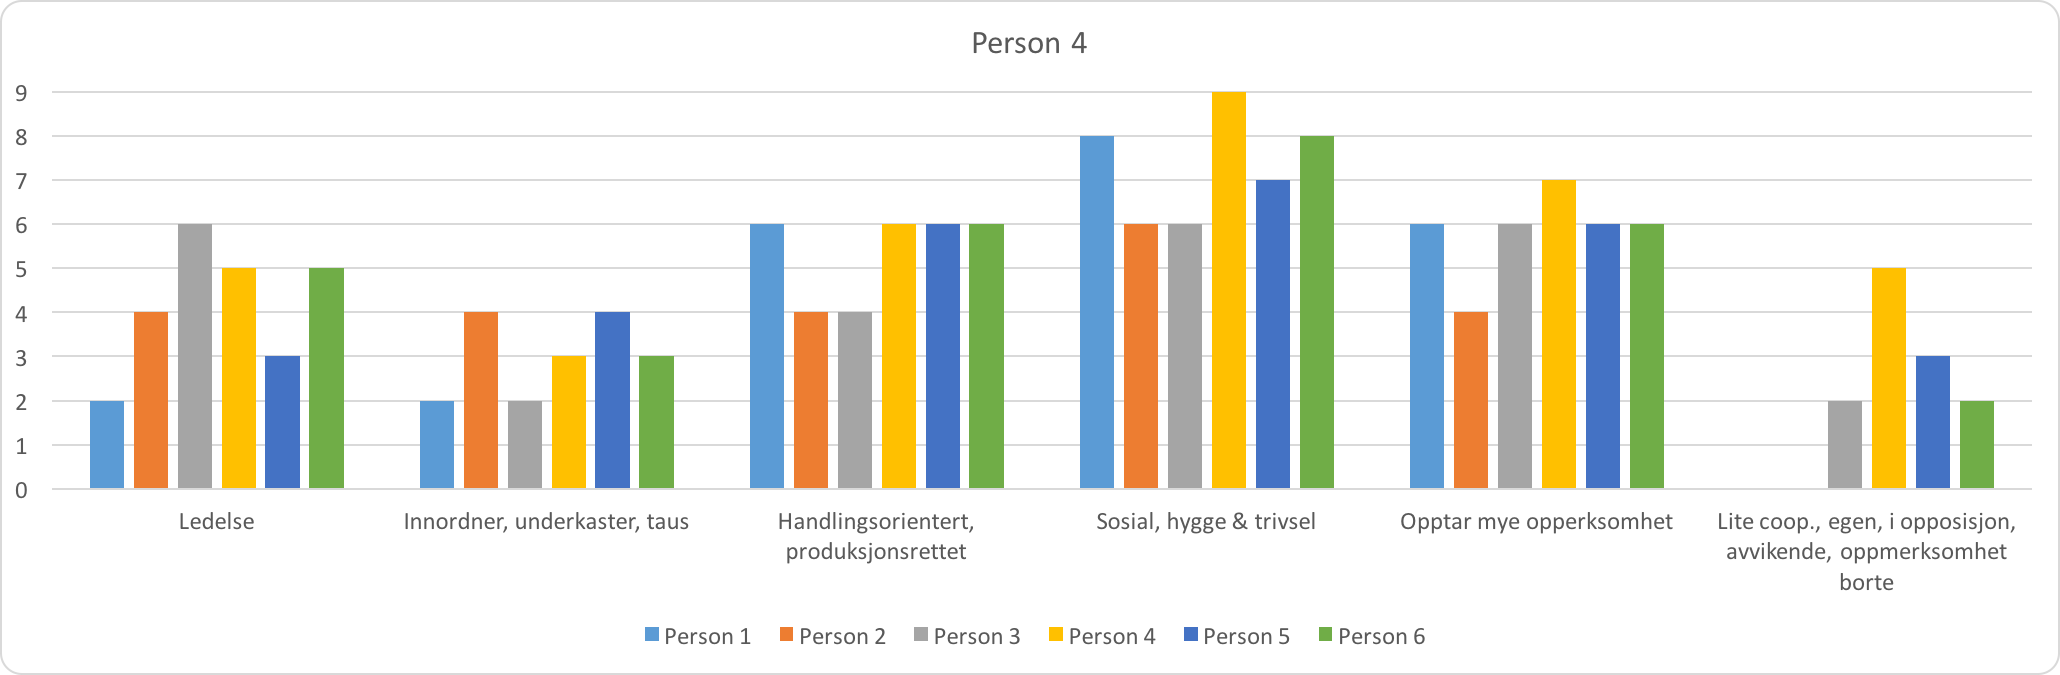
\includegraphics[width=1\textwidth]{gfx/roller_person4.png}
\caption{Roller – Person 4}
\label{roller_person4}
\end{figure}

\begin{figure}[!ht]
\centering
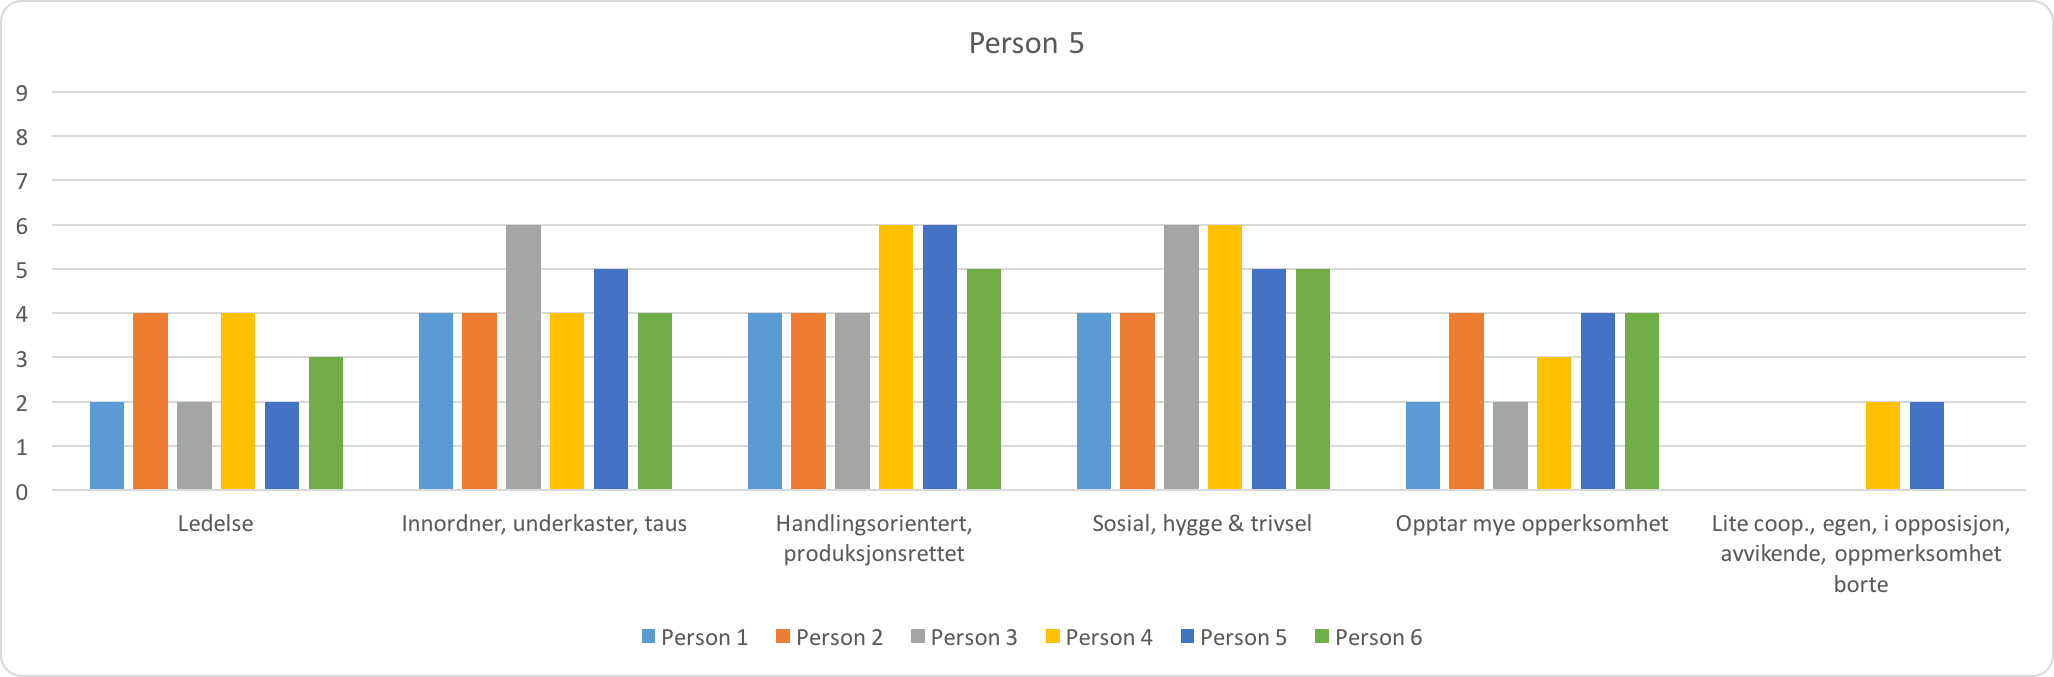
\includegraphics[width=1\textwidth]{gfx/roller_person5.png}
\caption{Roller – Person 5}
\label{roller_person5}
\end{figure}

\begin{figure}[!ht]
\centering
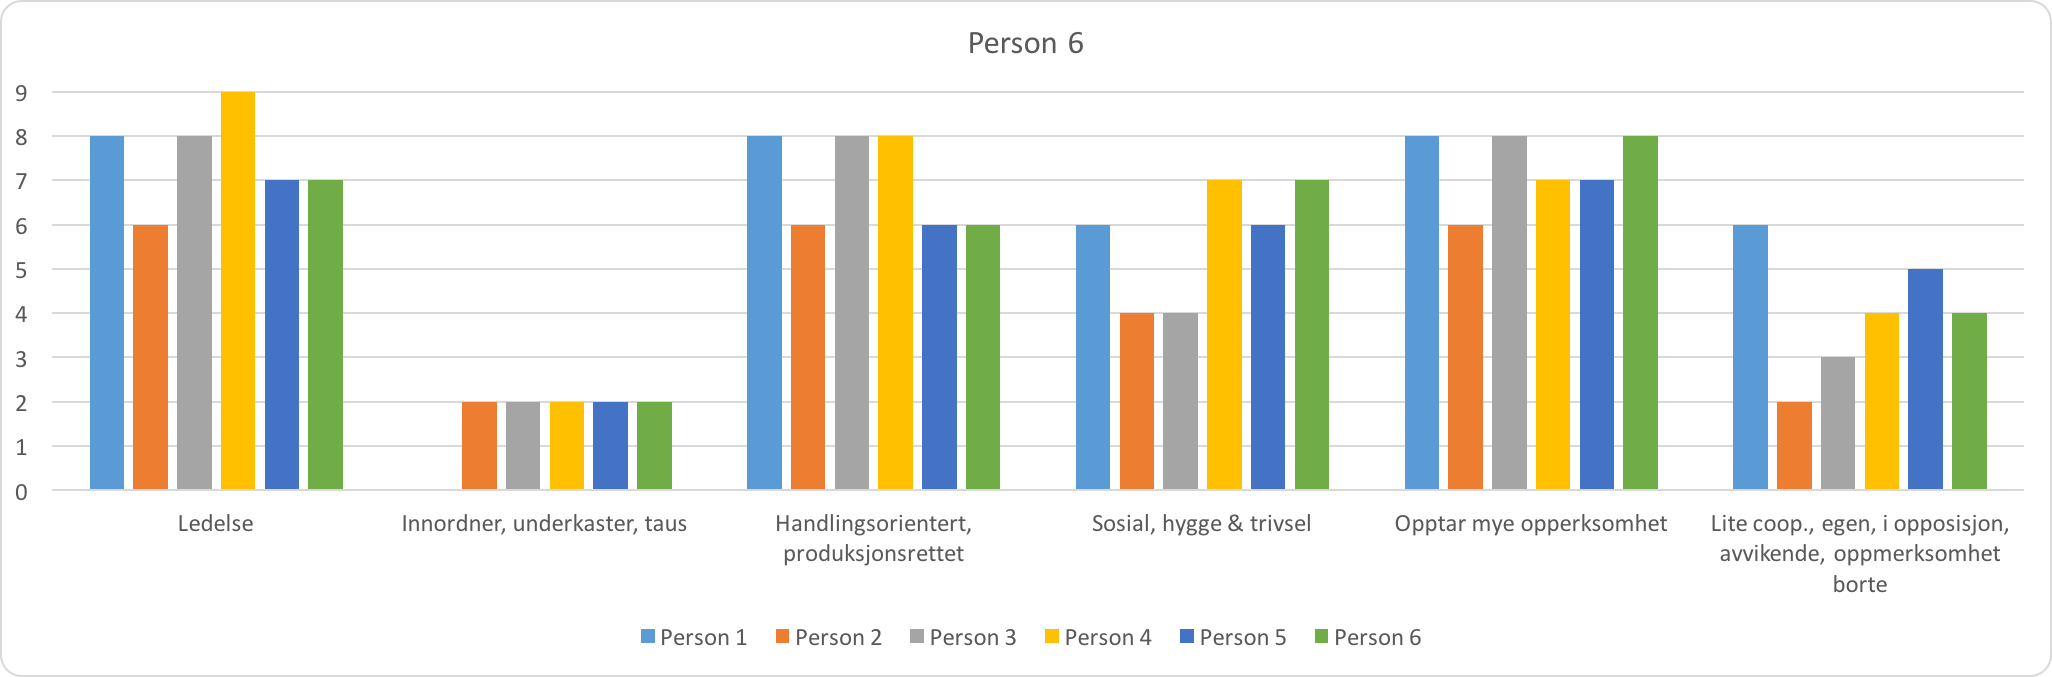
\includegraphics[width=1\textwidth]{gfx/roller_person6.png}
\caption{Roller – Person 6}
\label{roller_person6}
\end{figure} % Appendix A

%----------------------------------------------------------------------------------------
%	POST-CONTENT THESIS PAGES
%----------------------------------------------------------------------------------------

\cleardoublepage% Bibliography

\label{app:bibliography} % Reference the bibliography elsewhere with \autoref{app:bibliography}

\manualmark
\markboth{\spacedlowsmallcaps{\bibname}}{\spacedlowsmallcaps{\bibname}} 
\refstepcounter{dummy}

\renewcommand{\bibname}{Bibliografi}

\addtocontents{toc}{\protect\vspace{\beforebibskip}} % Place the bibliography slightly below the rest of the document content in the table of contents
\addcontentsline{toc}{chapter}{\tocEntry{\bibname}}

\bibliographystyle{unsrtnat}

\bibliography{Bibliography} % Bibliography

\cleardoublepage\include{FrontBackMatter/Colophon} % Colophon

\cleardoublepage\include{FrontBackMatter/Declaration} % Declaration

%----------------------------------------------------------------------------------------

\end{document}
